\NeedsTeXFormat{LaTeX2e}[2005/12/01]
%%    2009/03/12 v1.0 GAUBM Vorlage für Aschlussarbeiten Physik
%% Template fuer Bachelor- und Masterarbeiten
%% an der Fakultaet fuer Physik (c) Thomas Pruschke der GA Universität
%% Verbesserungsvorschlaege bitte an studiendekanat@physik.uni-goettingen.de
%%
%% Benoetigte Pakete: datenumber
%%

%%%%%%%%%%%%%%%%%%%%%%%%%%%%%%%%%%%%%%%%%%%%%%%%%%%%%%%%%%%%%%%%%%%%%%
%%%%%%%%%% Bitte vor dem Veraendern diese Datei umbenennen! %%%%%%%%%%
%%%%%%%%%%%%%%%%%%%%%%%%%%%%%%%%%%%%%%%%%%%%%%%%%%%%%%%%%%%%%%%%%%%%%%

%% scrbook - Ersatz für LaTeX book Klasse aus dem KOMA Script
%% Moegliche Optionen: diejenigen der Klasse scrbook ausser titlepage

%% deutsche Arbeit:
\documentclass[bachelor,       %% Typ der Arbeit: bachelor oder master
               twoside,        %% zweiseitiges Layout
               BCOR10mm,       %% Bindekorrektur 10 mm
%               liststotoc,nomtotoc,bibtotoc, %% Aufnahme der div. Verzeichnisse
                                              %% ins Inhaltsverzeichnis
               ngerman, english %% Alternativspr. Englisch, Dokumentspr. Deutsch
%               ngerman,english  %% Alternativspr. Deutsch, Dokumentspr. Englisch
%               final,          %% Endversion; draft fuer schnelles Kompilieren
               ]{GAUBM}

\usepackage{graphicx}
\usepackage{caption}
\usepackage{subcaption}
\usepackage{algorithm}
\usepackage{algpseudocode}
\usepackage{csquotes}
\usepackage[printonlyused, withpage, smaller]{acronym}
\usepackage{setspace}  %% Zur Setzung des Zeilenabstandes
\usepackage{babel}     %% Sprachen-Unterstuetzung
\usepackage{calc}      %% ermoeglicht Rechnen mit Laengen und Zaehlern
\usepackage[T1]{fontenc}       %% Unterstutzung von Umlauten etc.
\usepackage[latin1]{inputenc}  %% 
%% in aktuellem Linux & MacOS X wird standardmaessig UTF8 kodiert!
%\usepackage[utf8]{inputenc}    %% Wenn latin1 nicht geht ...

\usepackage{amsmath,amssymb} %% zusaetzliche Mathe-Symbole

\usepackage{lmodern} %% type1-taugliche CM-Schrift als Variante zur
                     %% "normalen" EC-Schrift
%% Paket fuer bibtex-Datenbanken
\usepackage[comma,numbers,sort&compress]{natbib}
\bibliographystyle{plainnat}

\newcommand{\tabheadfont}[1]{\textbf{#1}} %% Tabellenkopf in Fett
\usepackage{booktabs}                      %% Befehle fuer besseres Tabellenlayout
\usepackage{longtable}                     %% umbrechbare Tabellen
\usepackage{array}                         %% zusaetzliche Spaltenoptionen

%% umfangreiche Pakete fuer Symbole wie \micro, \ohm, \degree, \celsius etc.
\usepackage{textcomp,gensymb}

%\usepackage{SIunits} %% Korrektes Setzen von Einheiten
\usepackage{units}   %% Variante fuer Einheiten

%% Hyperlinks im Dokument; muss als eines der letzten Pakete geladen werden
\usepackage[pdfstartview=FitH,      % Oeffnen mit fit width
            breaklinks=true,        % Umbrueche in Links, nur bei pdflatex default
            bookmarksopen=true,     % aufgeklappte Bookmarks
            bookmarksnumbered=true  % Kapitelnummerierung in bookmarks
            ]{hyperref}

%% Weiter benoetigte Pakete: datenumber
%% Falls dieses Paket nicht in der Installation vorhanden ist,
%% kann es von der Seite mit diesem Template heruntergeladen werden
%% und in einem LaTeX bekanntem Verzeichnis installiert werden (notfalls
%% dem Verzeichnis mit der Arbeit).
\begin{document}
%%
%%                   Ab hier muessen die Anpassungen geschehen
%%
%% Hier den eigenen Namen einsetzen
\ThesisAuthor{Justus}{Multhaup}
%% Hier den Geburtsort einsetzen
\PlaceOfBirth{Holzminden}
%% Titel Arbeit. Das erste Argument ist der deutsche, das zweite der
%% englische Titel.
\ThesisTitle{Teilchensimulationen von Polymermischungen in begrenzten Geometrien mit zeitabh\"angigen Randbedinungen}{Particle simulations of polymer mixtures in confined geometries with time dependent boundary conditions}
%% Erst- und Zweitgutacher/in
%% Ist der/die Betreuer/in nicht identisch mit dem/r Erstgutachter/in,
%% muss diese/r als optionales Argument angegeben werden.
\FirstReferee{Prof. Dr. Marcus M\"uller}
\Institute{Institut f\"ur Theoretische Physik}
\SecondReferee{Prof. Dr. Stefan Klumpp}
%% Beginn und Ende des Anfertigungszeitraumes
\ThesisBegin{1}{4}{2023}
\ThesisEnd{30}{6}{2023}
%% DO NOT TOUCH THESE LINES!!!!
\frontmatter
\maketitle
\cleardoublepage
%% Zusammenfassung. Falls nicht gewuenscht, bitte auskommentieren.
% \begin{abstract}
%   Hier werden auf einer halben Seite die Kernaussagen der Arbeit
%   zusammengefasst.
% %% Optional: Stichwoerter. Wenn nicht gewuenscht, koennen die beiden
% %% folgenden Zeilen geloescht werden
%   \bigskip\par
%   \textbf{Stichw\"orter:} Physik, Bachelorarbeit
% \end{abstract}
%% So laesst sich in die andere Sprache umschalten (Englisch bzw. Deutsch)
% \begin{otherlanguage}{english}
% \begin{abstract}
%   Here the key results of the thesis may be presented in about
%   half a page.
%   \bigskip\par
%   \textbf{Keywords:} Physics, Bachelor thesis
% \end{abstract}
% \end{otherlanguage}

%% Ende des Vorspanns
\cleardoublepage
%% Ab hier 1 1/2 facher Zeilenabstand (durch setspace-Paket)
\onehalfspacing
%% Erzeugt Inhaltsverzeichnis
\tableofcontents

%% Hier kann man seine Bezeichnungsweisen erklaeren. Falls nicht
%% benoetigt, bis einschliesslich \end{nomenclature} auskommentieren
\begin{nomenclature}
%% Fuer die Berechnung der Spaltenbreiten muss \usepackage{calc}
%% geladen sein!
\section*{Acronyms}
\noindent
\begin{acronym}[SOMA]
 \acro{GPU}{Graphics processing unit}
 \acro{MC}{Monte-Carlo}
 \acro{MD}{Molecular Dynamics}
 \acro{NESS}{non-equilibrium steady state}
 \acro{SA}{Simulated Annealing}
 \acro{SCFT}{Self-Consistent Field Theory}
 \acro{SCMF}{Single-Chain-in-Mean-Field}
 \acro{SD}{Steepest descent}
 \acro{SMC}{Smart Monte-Carlo}
 \acro{SOMA}{SOft coarse-grained Monte-Carlo Acceleration}
 \acro{SSL}{Strong-segregation limit}
 \acro{WSL}{Weak-segregation limit}

 
\end{acronym}
\end{nomenclature}
%% \listoftables und \listoffigures sollten nur bei genuegender Anzahl Tabellen
%% verwendet werden
%\listoffigures
%\listoftables

\mainmatter   %% Anfang Hauptteil


\chapter{Introduction}
\begin{itemize}
    \item Still the old version from Einfuehrung ins Wissenschaftliche Arbeiten
\end{itemize}
Polymers are highly versatile macromolecules composed of repeating units called monomers. Their importance for life on earth cannot be overstated, biological polymers are involved in countless chemical reactions in the human body and form the backbone of proteins and DNA. Synthetic polymers are applied almost everywhere in modern society, ranging from simple packaging materials to highly sophisticated materials used in aerospace engineering. This is owed to their vast range of unique physical properties, such as high elasticity, flexibility and durability. When creating novel materials with very precise features, understanding how polymers interact with one another and form structure via phase separation in multicomponent systems is essential.\\
One important class of polymers is the so-called homopolymer, which is made of a single type of monomer unit, for example, polyethylene. Copolymers, in contrast, consist of two or more different types of monomer units. Copolymers that are concatenations of homopolymers of different types and lengths are called block-copolymers. One of the most interesting and extensively studied properties of copolymers is their ability to self-assemble into microphases \cite{leibler1980theory}. An important tool in understanding the mechanisms behind this microphase separation, and many other interesting properties, is the use of computer simulations. These include particle-based \ac{MD} and \ac{MC} methods as well as continuum-model-based and hybrid methods \cite{Shuanhu2017}. Particle-based simulations accurately model small-scale phenomena. However, despite rapid advancements in computer technology and high parallelizability, they are too computationally expensive to simulate long time scales since they involve the explicit calculation of the strong, bonded interactions between particles. This also poses limitations on the system size; macro scale phenomena are hard to capture. Continuum models, on the other hand, are less computationally expensive, but at the cost of a lower accuracy on the microscale. On the mesoscale, good agreement between the two types of models was observed, e.g. in the orientation of cylindrical mesophases upon solvent evaporation \cite{Dreyer22}. To evaluate the accuracy of continuum models on small-length scales, it is necessary to compare them to established particle-based models. One approach to this is to consider a simulation box in a particle-based simulation as a small section from a large continuum-model-based simulation. The dynamics are then driven by extracting the time evolution of the density fields at the boundaries from the continuum simulation and applying them in the particle-based simulation, e.g. employing non-periodic boundary conditions. However, dictating the boundary densities in particle-based simulations is not a trivial task. One option is the use of external fields or the umbrella sampling method \cite{glenn74}, although this has the large drawback that the number of particles in the simulation box remains constant, while in the continuum simulation particles can enter and leave the section at any time. An alternative is to employ conversion zones at the boundaries, in which molecules are converted to different types, mimicking particle exchange with the surrounding as shown in Figure \ref{fig:continuum_section}. If the densities are defined on a discretized grid, this leads to an optimization problem in which the ideal configuration of molecule types needs to be found, such that the mean squared deviation from the target density is minimized. \\
In this study, as a first step towards boundary-driven particle simulations, the dynamics of noninteracting homopolymers are investigated. Specifically, a system is pushed away from equilibrium by introducing conversion zones at the boundary regions of the simulation box. This results in a diffusive current and allows the calculation of the collective diffusion coefficient of the system. To this end, the \ac{SOMA} \cite{Schneider_soma} software package based on the \ac{SCMF} algorithm \cite{Daoulas06} is employed.
\begin{figure}[h]
  \centering
  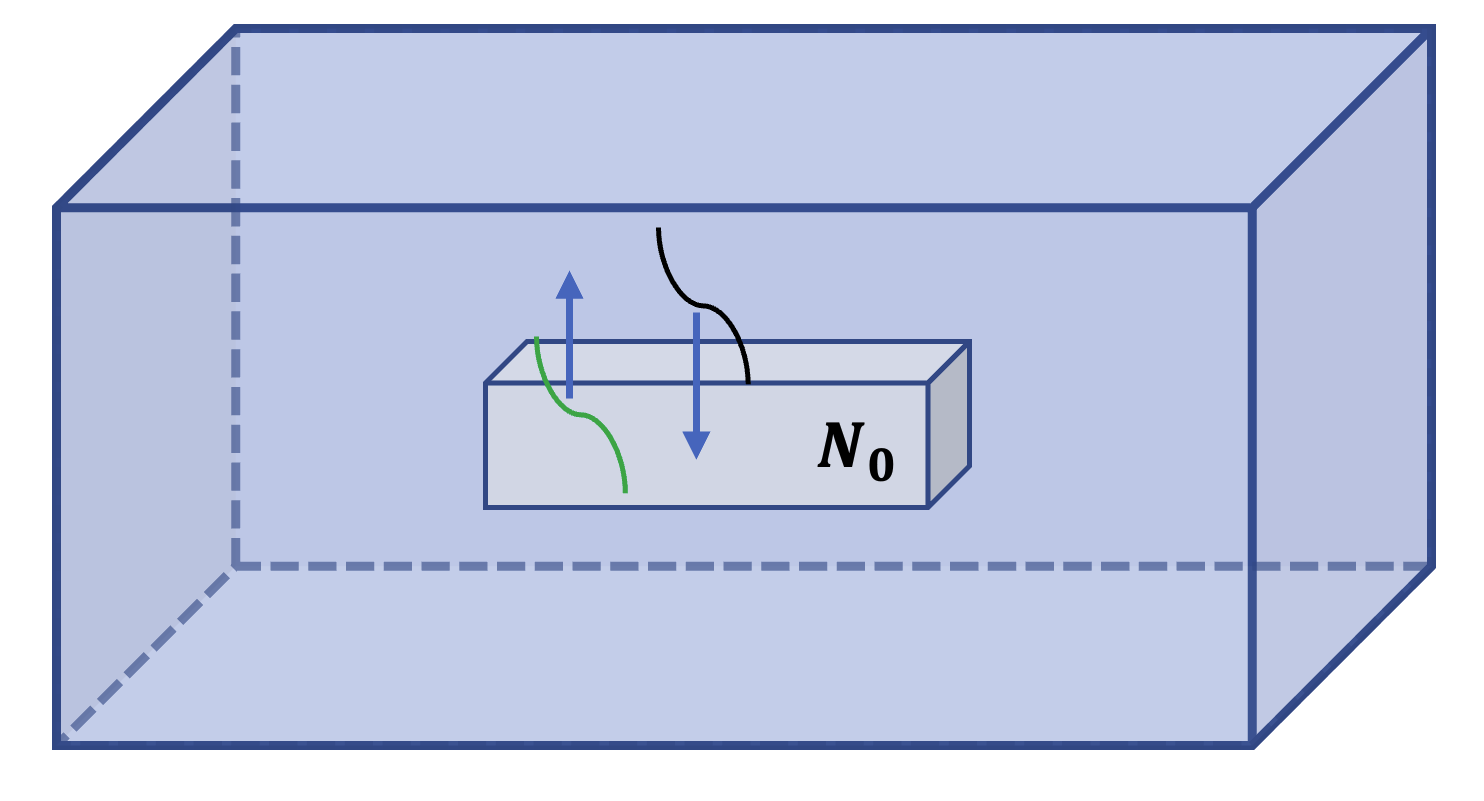
\includegraphics[width=0.6\linewidth]{figures/continuum_section.png}
  \caption{Sketch of the setting explained in the text. Polymers of different types may be exchanged with the surrounding, but the number of molecules $N_0$ inside the section of the particle simulation remains constant.}
  \label{fig:continuum_section}
\end{figure}



\chapter{Theory}

\section{Single-chain properties}

Since the collective dynamics of polymer mixtures can often be directly related to the single-chain properties, some selected aspects are briefly discussed here. The simplest model to describe a polymer chain is the ideal chain, for which any non-bonded interaction between monomers is neglected.
\subsection{The freely jointed chain}

The freely jointed chain model is an ideal model in which the chain is composed of $N$ segments of length $a\,,$ whose orientation vectors $\mathbf r_i$ ($a=|\mathbf r_i|$) can face in any direction and are completely independent from each other. The chain configuration may be characterised by the \textit{end-to-end-vector} $\mathbf R$:

\begin{align}
    \mathbf R=\sum_{i=1}^{N}\mathbf r_i\,.
\end{align}

Due to the completely random orientation, $\mathbf R$ has zero mean. A useful property to quantify the spatial extension of the chain is the mean square of $\mathbf R\,,$ which calculates to:

\begin{align}
    R_e^2\equiv \langle\mathbf R^2\rangle=Na^2\,.
\end{align}

For large $N\,,$ $\mathbf R$ has a Gaussian distribution \cite{Rubin03}:
 
 
\begin{align}
    P(N,\mathbf R)=\left(\frac{3}{2\pi R_e^2}\right)^{3/2}\exp\left[-\frac{3\mathbf R^2}{2R_e^2}\right]\,,
\end{align}
 
 the freely jointed chain therefore converges towards the Gaussian chain. 
 
\subsection{Rouse model}

The Rouse model \cite{Rouse} is used to describe the dynamics of a Gaussian chain moving through a solvent. The stiff bonds are replaced by springs of root-mean-square size $b\,,$ through which a monomer interacts with its neighbours. The monomers experience a friction force with friction coefficient  $\zeta\,,$ and the total friction coefficient of the center of mass is:

\begin{align}
    \zeta_\mathrm R=N\zeta\,.
\end{align}

Within the Rouse model, the diffusion coefficient of the chain is computed as:

\begin{align}
    D_\mathrm R=\frac{k_BT}{\zeta_\mathrm R}=\frac{k_BT}{N\zeta}\,.
    \label{eq:d_rouse}
\end{align}

For an $n$-dimensional diffusion of a Brownian particle, the single chain diffusion constant is related to the mean squared displacement of the chain center of mass $g_3(t)$ by the Einstein relation \cite{einstein_1905}:

\begin{align}
    D&=\frac{g_3(t)}{2nt}\,,\\
    g_3(t)&=\langle (\mathbf r_{cm}(t)-\mathbf r_{cm}(t_0))^2\rangle\,,\nonumber
    \label{eq:einstein_relation}
\end{align}

where $\mathbf r_{cm}(t)$ is the center of mass position at time $t$ and $t_0$ is the time at which the measurement is started. The time in which a polymer diffuses a distance of the order of its size is called relaxation time $\tau_\mathrm R\,$:

\begin{align}
    \tau_\mathrm R\approx\frac{R_e^2}{D_\mathrm R}=\frac{\zeta}{k_BT}{NR_e^2}\,.
\end{align}

On time scales larger than $\tau_\mathrm R\,,$ the chain movement is only due to diffusion, while viscoelastic effects are observed at shorter time scales. 
 
 
\section{Polymeric mixtures}
Polymer mixtures consist of two or more chemically different polymer types. The mechanical and thermodynamic properties can vary greatly with several factors such as composition, molecular weight and interactions between the polymers. This makes them desirable for manufacturing materials with tailored properties.\\
If the composition is uniform everywhere, the mixture is called homogeneous. In a heterogeneous mixture, in contrast, the composition is non-uniform, leading to visible boundaries which may have very different properties. This phenomenon is also called macro-phase separation. From an entropic viewpoint, mixing is always favored. However, energetic interactions between polymers may either favor or suppress mixing. Whether a mixture is homogeneous or heterogeneous, thus,  depends on the balance between entropy and energy \cite[S. 137]{Rubin03}.           

\subsection{Flory-Huggins Theory}

Whether mixing or phase separation will be favored can be predicted by determining the free-energy change associated with mixing the components. This free energy-change can be computed within the lattice model developed by Flory and Huggins \cite{Flory42}. Within the Flory-Huggins framework, no volume change is assumed upon mixing. With this assumption, it is convenient to represent the system on a lattice. A lattice site corresponds to the smallest molecular unit and every macromolecule takes up one or multiple lattice sites. Consider a binary mixture with $n_\mathrm A$ polymers of species A and chain length $N_\mathrm A$ and $n_\mathrm B$ polymers of species B and chain length $N_\mathrm B$. Let the total number of polymers be $n=n_\mathrm A+n_\mathrm B\,.$ The free energy of mixing per monomer $\Delta F_{mix}$ is then given by the Flory-Huggins equation of polymer solutions \cite[S. 143]{Rubin03}:

\begin{align}
  \frac{\Delta F_{mix}}{k_BT}=\frac{\phi}{N_\mathrm A}\ln\phi+\frac{1-\phi}{N_\mathrm B}\ln(1-\phi)+\chi\phi(1-\phi)\,.
  \label{eq:floryhuggins}
\end{align}

Here, $\phi=n_\mathrm AN_\mathrm A/(n_\mathrm AN_\mathrm A+n_\mathrm BN_\mathrm B)$ is the monomer fraction of species A, $k_B$ is the Boltzmann constant, $T$ is the system temperature and $\chi$ is the Flory interaction parameter which characterizes the interaction between different polymer species and can be obtained from experiments. A positive value of $\chi$ opposes mixing while a negative value promotes it; knowing the value of $\chi$, therefore, allows us to qualitatively predict the phase separation behavior. For $\chi=0\,,$ \eqref{eq:floryhuggins} reduces to regular solution theory for an ideal gas of polymers with concentrations $\phi/N_A$ and $(1-\phi)/N_B\,.$  Note that so far, no space dependency of $\phi$ has been assumed. In the following discussion, a symmetric mixture with $N_\mathrm A=N_\mathrm B=N$ is assumed. To fully capture the complexity of the system, the Flory-Huggins model has to be extended to include spatial variations of $\phi$, which gives rise to the de Gennes-Flory-Huggins free-energy functional  \cite{deGennes80, Reister02}:


\begin{align}
  \frac{F[\phi]R_e^3}{k_BT\sqrt{\bar N}}=\int \mathrm{d}^3\mathbf{r}\left\{\phi\ln\phi+(1-\phi)\ln(1-\phi)+\chi N\phi(1-\phi)+k(\phi)[\nabla\phi]^2\right\}\,.
  \label{eq:flory_fctl}
\end{align}

Here, $\bar N=\left(nR_e^3/V\right)^2$ is the invariant degree of polymerization of the system with volume $V$. It is a measure of the number of neighboring chains a chain interacts with. The term proportional to $[\nabla\phi]^2$ is added to the free-energy density to ensure that unphysical, sharp changes in the local densities are penalized. The precise form of $k(\phi)$ depends on the strength of the parameter $\chi\,$. For small $\chi N\lesssim 5\,,$ one considers the \ac{WSL}. For large $\chi N\gtrsim10\,$ \cite{Semenov1996Dec}, the \ac{SSL} holds. In these two limits, the prefactor $k$ takes the following form \cite{Reister02}:

\begin{align}
  k_\mathrm{WSL}=\frac{R_e^2}{36\phi(1-\phi)}\,;\qquad k_\mathrm{SSL}=\frac{R_e^2}{24\phi(1-\phi)}\,.
\end{align}


\section{Collective diffusion}

Consider again a binary mixture of polymers with $N_\mathrm A=N_\mathrm B=N\,$. Since the number of polymers in the system is constant, the continuity equation holds:

\begin{align}
  \frac{\partial\phi}{\partial t}+\nabla\cdot\mathbf{J}_\mathrm A=0\,.
  \label{eq:conti}
\end{align}

Here, $\mathbf{J}_\mathrm A$ is the local current of polymer species A. Near equilibrium, one postulates a linear relation between $\mathbf{J}_\mathrm A$ and the local chemical potential $\mu_\mathrm A$ \cite{deGennes80}. In the most general case, this relation is non-local in space and time. Assuming translational invariance in space and time, it reads \cite{erukhimovich1986nonexponential}:


\begin{align}
    \mathbf{J}_\mathrm A(\mathbf{r},t)=-\int_{t'=-\infty}^t\mathrm d t'\int_V\mathrm d \mathbf{r'}\,\frac{\Lambda_\mathrm A(\mathbf{r}- \mathbf{r'},t-t')}{k_BT}\nabla '\mu_\mathrm A(\mathbf{r'},t')\,.
    \label{eq:linear_response}
\end{align}

The Onsager coefficient $\Lambda_\mathrm{A}(\mathbf{r}- \mathbf{r'},t-t')$ relates the gradient of the chemical potential at position $\mathbf{r'}$ to a density flux at position $\mathbf r$ and also accounts for memory effects. The non-localities in \eqref{eq:linear_response} translate into a dependency of $\Lambda$ on the wave vector $\mathbf q$ and the frequency $\omega$ in Fourier space. In the time-independent steady state, this gives:


\begin{align}
    \mathbf {J}_{\mathrm A, q}=-iq\frac{\Lambda_{\mathrm A, q}}{k_BT}\mu_{\mathrm A, q}\,,
\end{align}

where $q=|\mathbf q|\,.$ In the following, it is assumed that $\mu[\phi(x)]\propto x\,,$ so $\mu_q\propto 1/q$ and $\nabla\mu=\mathrm{const}\,.$ For a spatially independent current, this implies that $\Lambda$ must also be independent of $q\,,$ so in the spatial picture: 


\begin{align}
    \mathbf {J}_\mathrm A=-\frac{\Lambda_\mathrm A}{k_BT}\nabla\mu_\mathrm A\,.
    \label{eq:current_local}
\end{align}


This approximation holds for small $q$ and therefore prohibits the probing of the $q$-dependence of $\Lambda\,,$ but it leads to a simple form of the Onsager coefficient that will be derived in the following. 

%%  Derivation in Binder paper

% Following the discussion in the appendix of \cite{Binder83}, a continuity equation can be written down for each type individually:

% \begin{align}
%   \frac{\partial\phi_\mathrm A}{\partial t}+\nabla\cdot\mathbf{J_A}=0\,; \qquad \frac{\partial\phi_\mathrm B}{\partial t}+\nabla\cdot\mathbf{J_B}=0\,.
%   \label{eq:conti_ab}
% \end{align}

% With the additional assumption of incompressibility, e.g. $\rho(\mathbf{r},t)\equiv\phi_\mathrm A(\mathbf{r},t)+\phi_\mathrm B(\mathbf{r},t)=1$ everywhere for all times, the continuity equation for the total density $\rho$ separates into two distinct equations:

% \begin{align}
%   \frac{\partial}{\partial t}(\phi_\mathrm A+\phi_\mathrm B)=0\,; \qquad \nabla\cdot (\mathbf{J_A}+\mathbf{J_B})=0  \,.
% \end{align}

% This implies that $\mathbf{J_A}=-\mathbf{J_B}\,,$ which simply reflects the condition of incompressibility: for a bead of type A to move, a bead of type B has to take its place and vice-versa. The Onsager relations are then
% \begin{subequations}
%   \begin{align}
%     \mathbf{J_A}&=-\frac{\Lambda_{\mathrm{AA}}}{k_BT}\nabla\mu_\mathrm A\,,\\
%     \mathbf{J_B}&=-\frac{\Lambda_{\mathrm{BB}}}{k_BT}\nabla\mu_\mathrm B\,,
%     \label{eq:current_onsager}
%   \end{align}
% \end{subequations}


% where $\Lambda_\mathrm{AA}$ and $\Lambda_\mathrm{BB}$ are the diagonal elements of the matrix of Onsager coefficients, which is assumed to be diagonal. Since $\mu_\mathrm A$ and  $\mu_\mathrm B$ are not independent variables, their difference $\Delta\mu=\mu_\mathrm A-\mu_\mathrm B$ is considered instead. The goal is now to relate $\Delta\mu$ to the current $\mathbf J(\mathbf r,t)=\mathbf {J_A}(\mathbf r,t)=-\mathbf {J_B}(\mathbf r,t)\,.$ From \eqref{eq:current_onsager}, it is easily seen that

% \begin{align}
%   \nabla(\mu_\mathrm A-\mu_\mathrm B)&=-k_BT\left (\mathbf{J_A}\Lambda_{\mathrm{AA}}^{-1} - \mathbf{J_B}\Lambda_{\mathrm{BB}}^{-1}\right )\nonumber\\
%   &=-k_BT\left (\Lambda_\mathrm{AA}^{-1}+\Lambda_\mathrm{BB}^{-1}\right )\mathbf{J}
% \end{align}

% and therefore

% \begin{align}
%   \mathbf J=-\frac{1}{k_BT}\left (\Lambda_\mathrm{AA}^{-1}+\Lambda_\mathrm{BB}^{-1}\right )^{-1}\nabla(\mu_\mathrm A-\mu_\mathrm B)\,.
% \end{align}

% The Onsager coefficient that relates $\mathbf{J}$ to the local chemical potential difference is identified as $\Lambda^{-1}=\Lambda_\mathrm{AA}^{-1}+\Lambda_\mathrm{BB}^{-1}\,.$ By relating the currents in \eqref{eq:current_onsager} to the single chain diffusion coefficients $D_A$ and $D_B\,,$ the Onsager coefficients may be identified as $\Lambda_\mathrm{AA}=N_\mathrm AD_A\phi$ and $\Lambda_\mathrm{BB}=N_\mathrm BD_B(1-\phi)\,.$ For a symmetric mixture with $N_\mathrm A=N_\mathrm B\equiv N $ and $D_A=D_B\equiv D\,,$ the Onsager coefficient corresponding to $\Delta\mu$ becomes


% \begin{align}
%   \Lambda=DN\phi(\mathbf{r})(1-\phi(\mathbf{r}))\,.
%   \label{eq:onsager}
% \end{align}


% This result has also been derived by de Gennes \cite{deGennes80}.\\


%% Alternative derivation in de Gennes paper


Following the discussion in the appendix of \cite{deGennes80}, consider a mixture of polymer chains with densities $\phi_\mathrm A$ and $\phi_\mathrm B\,.$ Incompressibility, e.g. $\phi_\mathrm A+\phi_\mathrm B=1\,,$ is enforced by introducing an additional repulsive potential $U$ to the chemical potential, so from \eqref{eq:current_local} one obtains:



\begin{subequations}
  \begin{align}
    \mathbf{J}_\mathrm A&=-\Lambda_\mathrm A\nabla [(\mu_\mathrm A + U)/k_BT]\,,\\
    \mathbf{J_B}&=-\Lambda_\mathrm B\nabla [(\mu_\mathrm B + U)/k_BT]\,.
  \end{align}
  \label{eq:current_onsager}
\end{subequations}

Due to the incompressibility, the total current $\mathbf J=\mathbf{J}_\mathrm A+\mathbf{J}_\mathrm B$ must have zero divergence, which in one dimension means $\mathbf J\equiv J\mathbf{e_x}=\mathrm{const}\,.$ From the Galilei invariance of the system, we can simply choose $J=0\,.$ From this condition, $U$ can be calculated explicitly:

\begin{align}
  U=(\Lambda_\mathrm A\mu_\mathrm A+\Lambda_\mathrm B\mu_\mathrm B)/(\Lambda_\mathrm A+\Lambda_\mathrm B)\,.
\end{align}

Since one of the currents is redundant, write $J\equiv J_A\,.$ From \eqref{eq:current_onsager}, obtain:

\begin{align}
  J=-\Lambda\nabla(\mu_\mathrm A - \mu_\mathrm B)\equiv -\Lambda\nabla\mu\,,
\end{align}

where $\Lambda=\Lambda_\mathrm A\Lambda_\mathrm B/(\Lambda_\mathrm A+\Lambda_\mathrm B)$ and $\mu$ is the exchange chemical potential. In the limit of no interactions, the mixture can be considered as an ideal gas, so $\Lambda_i=D_i/\phi_i$ for $i=\mathrm A, \mathrm B\,.$ For $D_\mathrm A=D_\mathrm B\equiv D\,,$ this yields:

\begin{align}
  \Lambda=D\phi(\mathbf{r})(1-\phi(\mathbf{r}))\,.
  \label{eq:onsager}
\end{align}
This approximation is frequently used in the literature for the sake of computational efficiency \cite{Fraaje97,deGennes80,Binder83}. It corresponds to a local coupling in which monomers move like the center of mass, therefore it does not account for the connectivity of the monomers along the backbone of the chain. 

\section{Single chain in mean field simulations}


% First option following http://dx.doi.org/10.1063/1.2364506

Although the soft, coarse grained model used in this thesis provides a high flexibility in molecular architectures, the following discussion is restricted to symmetric  AB-diblock copolymers in a volume $V$ at temperature $T$ for simplicity. As usual, we first write down the partition function:

\begin{align}
    \mathcal{Z}\propto\frac{1}{n!}\int{\prod_{i=1}^n\mathcal{D}[\mathbf r_i(s)]\mathcal P_0[\mathbf r_i(s)]\exp\left(\frac{-\mathcal H_{\text{nb}}[\hat\phi_\text A,\hat\phi_\text B]}{k_BT}\right)}\,,
    \label{eq:partition_function}
\end{align}

where $\mathbf r_i(s)$ is the position of segment $s$ from molecule $i\,.$ The factor $\int\mathcal{D}[\mathbf r_i(s)]\equiv \int\prod_sd^3\mathbf r_i(s)$ integrates over the conformation space of molecule $i\,.$ Conformations are weighted by a Boltzmann factor $P_0[\mathbf r_i(s)]\propto\exp\left(-\mathcal H_{\text{b}}[\mathbf r_i(s)]/k_BT\right)$ that involves the bonded interactions in the abscence of any intermolecular interactions. The bonded interactions $\mathcal H_{\text{b}}[\mathbf r_i(s)]$ are modeled by harmonic potentials, which is appropriate for Gaussian polymers. The discretized form reads:

\begin{align}
    \frac{\mathcal H_\text b[\mathbf r_i(s)]}{k_BT}=\sum_{s=1}^{N-1}\frac{3(N-1)}{2R_e^2}[\mathbf r_i(s)-\mathbf r_i(s+1)]\,.
\end{align}

The non-bonded interactions $\mathcal H_\text{nb}$ in \eqref{eq:partition_function} depend on the local particle densities $\hat\phi_\text A$ and $\hat\phi_\text B$ and are modeled by the following excess interaction free energy functional:

\begin{align}
    \frac{\mathcal H_\text{nb}[\hat\phi_\text A,\hat\phi_\text B]}{k_BT}=\frac{\rho_0}{N}\int_Vd^3\mathbf r\left(\frac{\kappa N}{2}[\hat\phi_\text A+\hat\phi_\text B-1]^2-\frac{\chi N}{4}[\hat\phi_\text A-\hat\phi_\text B]^2\right)\,,
    \label{eq:nonbonded}
\end{align}

where $\rho_0=\frac{nN}{V}$ is the average monomer density. The first term in the integrand penalizes deviations of the total density from unity, and therefore controls the extent of density fluctuations with the control parameter $\kappa\,.$ The second term enforces the repulsion of monomers of different types with the control parameter $\chi\,.$ The densities $\hat\phi_{\alpha,m}$ ($\alpha=\text A,\text B$) are defined on a cubic grid with spacing $\Delta L\,,$ the total number of cells is $N_{cells}=V/(\Delta L)^3\,.$ They are obtained by summing over all beads and assigning them to their according cell:

\begin{align}
    \hat\phi_{\alpha,m}=\sum_{i=1}^n\sum_{s=1}^N\Pi(\mathbf r_i(s),\mathbf c_m)\gamma_\alpha(s)\,,
\end{align}

where $\gamma_\alpha(s)$ assigns the segments to their respective types: it is one if segment $s$ is of type $\alpha\,,$ and zero otherwise. $\Pi(\mathbf r_i(s),\mathbf c_m)$ is the characteristic function of the grid cell centered at $\mathbf c_m\,.$ This way, $\eqref{eq:nonbonded}$ may be discretized in the following way:

\begin{align}
    \frac{\mathcal H_\text{nb}[\hat\phi_\text A,\hat\phi_\text B]}{k_BT}=\frac{\rho_0\Delta L^3}{N}\sum_{m=1}^{N_{cells}}\left(\frac{\kappa N}{2}[\hat\phi_{\text A,m}+\hat\phi_{\text B,m}-1]^2-\frac{\chi N}{4}[\hat\phi_{\text A,m}-\hat\phi_{\text B,m}]^2\right)\,.
    \label{eq:nonbonded_discretized}
\end{align}

Since the non-bonded interactions vary on a time-scale that is much slower than the bonded interactions \cite{Daoulas06}, they are approximated by quasi-instantaneous external fields $\omega_{\alpha,m}$:

\begin{align}
    \omega_{\alpha,m}&=\frac{1}{k_BT\rho_0\Delta L^3}\frac{\partial \mathcal H_{\text{nb}}}{\partial \hat\phi_{\alpha,m}}\,,\nonumber \\
    \omega_{\text A,m}&=\kappa N\left(\hat\phi_{\text A,m}+\hat\phi_{\text B,m}-1\right)-\frac{\chi N}{2}\left(\hat\phi_{\text A,m}-\hat\phi_{\text B,m}\right)\,,
    \label{eq:calc_omegafields}
\end{align}

and similarly for $\omega_{\text B,m}\,.$ In the \ac{SCMF} algorithm, these external fields are kept constant over a short duration. A \ac{MC} scheme is used to update the particle positions. A trial move is proposed according to a predefined rule and accepted according to the Metropolis-Hastings criterion \cite{metropolis}:

\begin{align}
    p_{\text{acc}}=\min\left\{1\,,\exp\left(-\frac{\Delta E}{k_BT}\right)\right\}\,,
    \label{eq:metropolis_mc}
\end{align}

where $\Delta E=\Delta\mathcal H_{\text b}+\Delta\mathcal H_{\text{nb}}^{\text{SCMF}}$ is the energy change associated with the move. After a predefined number of \ac{MC} steps, the external fields are recalculated from the current densities. The accuracy of this approximation depends on the update frequency of the external fields as well as the parameter:

\begin{align}
    \epsilon =\frac{1}{\sqrt{N\bar{\mathcal N}}}\left(\frac{a}{\Delta L}\right)^3\,.
\end{align}



% Second option following http://dx.doi.org/10.1063/1.2364506
% Might be better because it is simpler and at the same time more general

% Within the soft, coarse grained model employed here, in principle, a great variety of molecular architectures can be implemented. For this reason, the term \enquote{macromolecule} will be frequently used in the following instead of \enquote{polymer}. The pairwise interaction energy associated with a bond $b$ of a molecule $m$ is $V_{m,b}(\mathbf r)\,.$
% Macromolecules, which are defined as a group of particles linked together by bonds, can take one of $m_t$ different molecular architectures. These architectures define the bond topology. The total bonded interactions are obtained by summation over all interactions of bonds $b$ in every molecule $m\,$: 

% \begin{align}
%     \frac{\mathcal H_\text b}{k_BT}=\sum_{m\in \text{\{mol\}}}\sum_{b\in {\text{\{bonds\}}}_m}V_{m,b}(\mathbf r)\,,
% \end{align}

% where $V_{m,b}(\mathbf r)$ is the interaction energy of a single bond and $\mathbf r$ denotes the distance vector between the two bond partners. Motivated by a coarse-graining of Gaussian chains, it is chosen as a harmonic potential:

% \begin{align}
%     V_{\text{harm}}(\mathbf r)=\frac{1}{2}k_0\mathbf r^2\,,
% \end{align}

% where $k_0$ is the spring constant. Each particle has one of $n_t$ different types, which dictate the non-bonded interactions. As done in the Self-Consistent Field Theory (SCFT) for multi-component polymer melts, these are defined as excess free energy functionals that depend on the local, normalised densities $\hat\phi_i(\mathbf r)$ with $i=0,\dots,n_t\,.$ These densities are defined on a cubic grid with linear spacing $\Delta L\,$:

% \begin{align}
%     \hat\phi_i(c)=\frac{1}{\Delta L^3\rho_0}\sum_{j\in\text{beads}}\Pi_c(\mathbf r_j)\delta_{\text{type}(j),i}\,,
%     \label{eq:density_grid}
% \end{align}

% where $\rho_0$ denotes the average number density of particles in the system and $\Pi_c(\mathbf r_j)=1$ if the $j$th bead is in cell $c$ and $\Pi_c(\mathbf r_j)=0$ otherwise. The non-bonded interactions are then defined as:

% \begin{align}
%     \frac{\mathcal H_{\text{nb}}[\{\hat\phi_i\}]}{k_BT}=\frac{\rho_0\Delta L^3}{N}\sum_{c\in\{\text{cells}\}}\left(\mathcal K_\text{fluc.}[\{\hat\phi_i(c)\}]+K_\text{inter.}[\{\hat\phi_i(c)\}]\right)\,.
% \end{align}

% Fluctuations of the total density are controlled by the term: 

% \begin{align}
%     \mathcal K_\text{fluc.}[\{\hat\phi_i(c)\}]=\frac{\kappa N}{2}\left(\sum_{i=0}^{n_t-1}\hat\phi_i(c)-1\right)^2\,,
% \end{align}

% where $\kappa$ is a model parameter that controls the compressibility. The second term,

% \begin{align}
%     \mathcal K_\text{inter.}[\{\hat\phi_i(c)\}]=-\sum_{i\neq j}\frac{\chi_{ij}N}{4}\left(\hat\phi_i(c)-\hat\phi_j(c)\right)^2\,,
% \end{align}

% controls the incompability between different types. The matrix $\chi_{ij}$ is a generalisation of the Flory-Huggins parameter to multi-component systems. The SCMF algorithm now exploits the fact that the non-bonded interactions are typically significantly weaker than the bonded interactions and temporal variations are slow. Instead of calculating them explicitly, they are approximated by quasi-instantaneous external fields, $\omega_i(c)\,,$ which are calculated as:

% \begin{align}
%     \omega_i(c)&=\frac{1}{k_BT\rho_0\Delta L^3}\frac{\partial \mathcal H_{\text{nb}}}{\partial \hat\phi_i(c)} \nonumber\\
%     &=\kappa\left(\sum_{i=0}^{n_t-1}\hat\phi_i(c)-1\right)-\sum_{k\neq i}\frac{\chi_{ik}}{2}\left(\hat\phi_i(c)-\hat\phi_j(c)\right)\,.
%     \label{eq:calc_omegafields}
% \end{align}


% In the SCMF algorithm, the particle  configuration at the current time step is used to compute the external fields, $\omega_i\,,$ given by  \eqref{eq:density_grid} and \eqref{eq:calc_omegafields}. Subsequently, the particles are subjected to these external fields and displaced according to a MC scheme, which involves the bonded interactions $\mathcal H_\text b$ and the SCMF interaction with the external field: 

% \begin{align}
%     \frac{\mathcal H_{\text{nb}}^\text{SCMF}}{k_BT}=\sum_{i=0}^{n_t-1}\sum_{c\in\{cells\}}\Delta L^3\rho_0\hat\phi_i(c)\omega_i(c)=\sum_{j\in\{beads\}}\omega_{\text{type}(j)}(c_j)\,,
% \end{align}

% where $c_j$ denotes the cell of particle $j\,.$


% \section{Smart Monte Carlo move}

% \begin{itemize}
%     \item to be extended
% \end{itemize}
% The friction from the Rouse model can be incorporated into MC simulations by using a Smart Monte Carlo (SMC) scheme \cite{SMC}. The particle positions are proposed according to:

% \begin{align}
%     \mathbf{r}_i'(s)=\mathbf{r}_i(s)+\frac{\Delta t}{\zeta}\mathbf F_i(\mathbf r)+\Delta \mathbf r\,,
% \end{align}

% where $\Delta \mathbf r$ is from the usual MC algorithm and $\mathbf F_i(s)$ is the bonded force acting on the segment. $\Delta t$ is the time step of the simulation and $\zeta$ controls the segmental friction. The value of $\Delta t\,,$ that maximizes the MC acceptance rate, was found to be $\Delta t=0.17(\zeta R_e^2/Nk_BT)\,$ \cite{mueller_deltat}.

\chapter{Simulation technique}
\begin{itemize}
    \item Still the old version from Einfuehrung ins Wissenschaftliche Arbeiten
\end{itemize}
To simulate the collective dynamics, a coarse-grained model of the polymers is employed. Within this model, several monomeric repeat units are grouped into an effective interaction center, called \textit{bead}, which allows for an efficient numerical implementation. Nevertheless, in this study, the terms \enquote{bead} and \enquote{monomer} will be used interchangeably. A great variety of universal properties of polymeric materials on mesoscopic length scales is accurately captured by coarse-grained models \cite{Baschnagel03}.\\
The software package that is used for the numerical calculations, \ac{SOMA} \cite{Schneider_soma}, uses a combination of a coarse-grained model and the \ac{SCMF} algorithm \cite{Daoulas06}. Unlike the widely used \ac{SCFT}, the \ac{SCMF} method includes fluctuation effects which are required to accurately describe certain systems and effects, e.g. dilute polymer solutions, the vicinity of phase transitions, or polymeric microemulsions \cite{Bates97, Mueller02, Schmid03}. Instead of calculating the interaction of a chain with all its surrounding explicitly, the chains are subjected to fluctuating external fields which are frequently recalculated from the density distribution. The densities are defined on a cubic grid. The time evolution of the system is then performed by \ac{MC} simulation and the external fields remain constant during one \ac{MC} sweep, this is called \textit{quasi-instantaneous field approximation}. The enormous benefit of this is that the chains are decoupled, making it possible to implement it effectively on parallel machines and leverage accelerators like Nivida \acp{GPU} \cite{Schneider_soma}. Additionally, \ac{SMC} scheme is employed that uses the strong bonded forces to propose a trial displacement resembling Brownian motion and produces Rouse-like dynamics \cite{Pangali78,Rossky78}.\\
While a full description of the \ac{SCMF} equations can be found in \cite{Daoulas06}, and will be omitted here, it is important to note that the interactions are fully described by three coarse-grained parameters: the average mean squared end-to-end distance $R_{e}^2$ of a chain in the absence of non-bonded interactions, the inverse thermal compressibility $\kappa_o N$ and the incompatibility between different bead types $\chi_o N$. The term \enquote{soft} in \ac{SOMA} relates to the soft nature of the non-bonded interactions, which arises from the systematic coarse-graining and allows for an overlap of beads \cite{Mueller11soft}.


\chapter{Collective diffusion of symmetric homopolymers}
\label{chap:colldiff}

\section{Reference system}

In this section, the collective diffusion properties of noninteracting homopolymers with $N_\mathrm A=N_\mathrm B=N$ and $\chi=0$ are investigated. As a reference system, a simulation box with $n=10000$ polymers and dimensions $L_x\times L_y\times L_z=9.75\times3\times3\,R_e^3$ is used, so the invariant degree of polymerization is $\sqrt{\bar{N}}\approx 114\,$. The spatial discretization is $\Delta L=0.125\,R_e\,$.  Periodic boundary conditions are applied in the lateral $y$ and $z$ directions, whereas impenetrable walls are applied in the $x$ direction. Initially, the polymers are distributed homogeneously in the system. To stimulate a flux in a \ac{NESS}, conversion zones of width $d=0.25\,R_e$ are introduced close to the walls. In each time step, if the center-of-mass coordinate $\mathbf r_{cm}$ of a polymer of type A lies in the left conversion zone, it is converted to type B with probability $p(A\rightarrow B)=r\,$. Analogously, conversion from B to A takes place in the right conversion zone with the same probability $r\,$. The current $\mathbf J$ is measured by tracking the number of polymer conversions. The simulation setup is depicted in Figure \ref{fig:simulation_box}. \\
The computation of the transport properties is complicated by boundary effects, such as a steep density drop close to the hard walls, which is of entropic origin. Furthermore, chains whose center of mass lies in the conversion zone may extend far beyond that zone. The range of these effects is approximated as $R_e$ and measurements are only taken in the region where the effects are negligible. 


\begin{figure}[h]
  \centering
  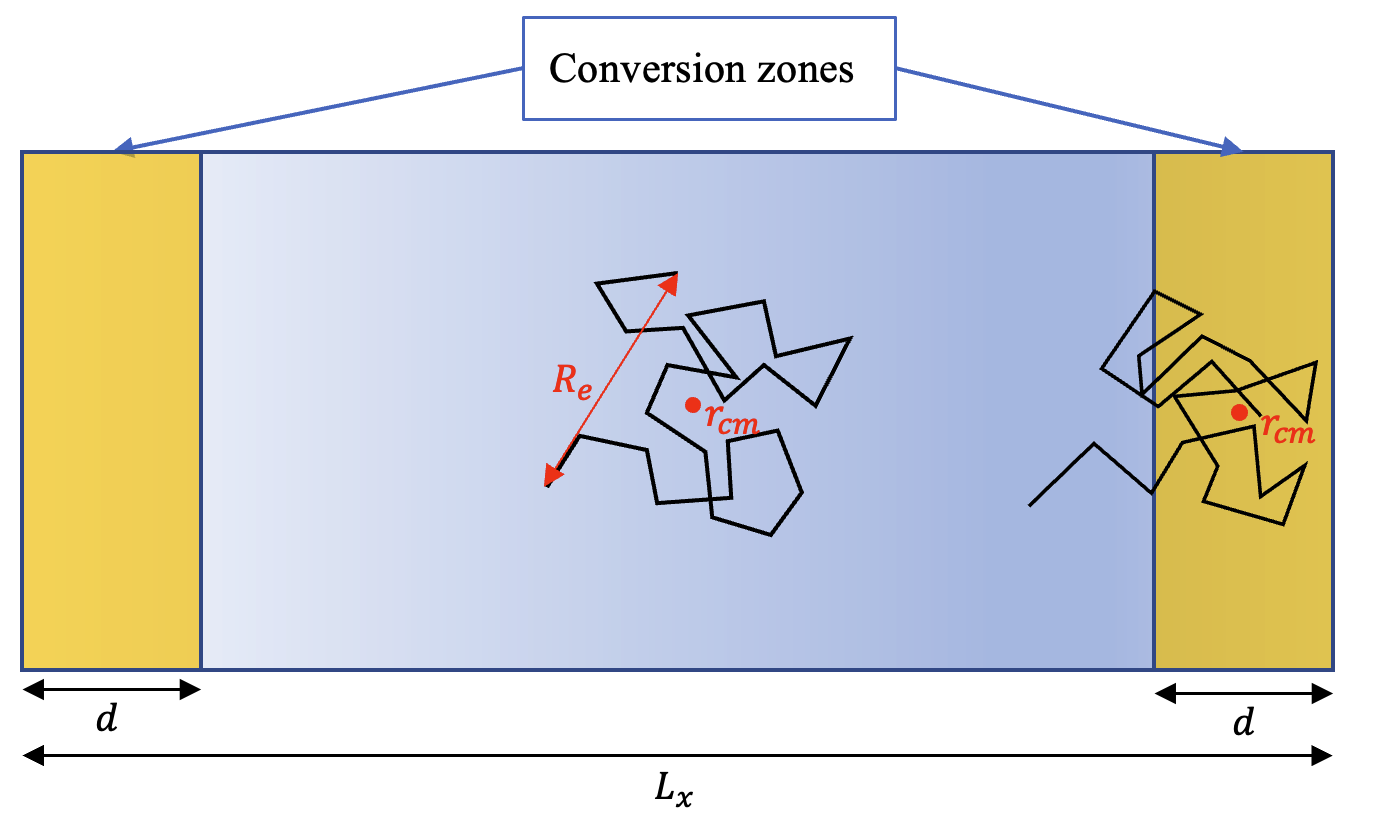
\includegraphics[width=0.7\linewidth]{figures/simulation_box.png}
  \caption{Simulation setup. For clarity, the conversion zones are not to scale and no distinction between polymer types is made.}
  \label{fig:simulation_box}
\end{figure}


\section{Collective diffusion coefficient}
\label{sec:colldiff}

Due to the periodic boundary conditions and the spatial homogeneity in the lateral directions, the system can effectively be described in one dimension. The density profile for $r=1.0$ is shown in Figure \ref{fig:density_profile}.

\begin{figure}[h]
  \centering
  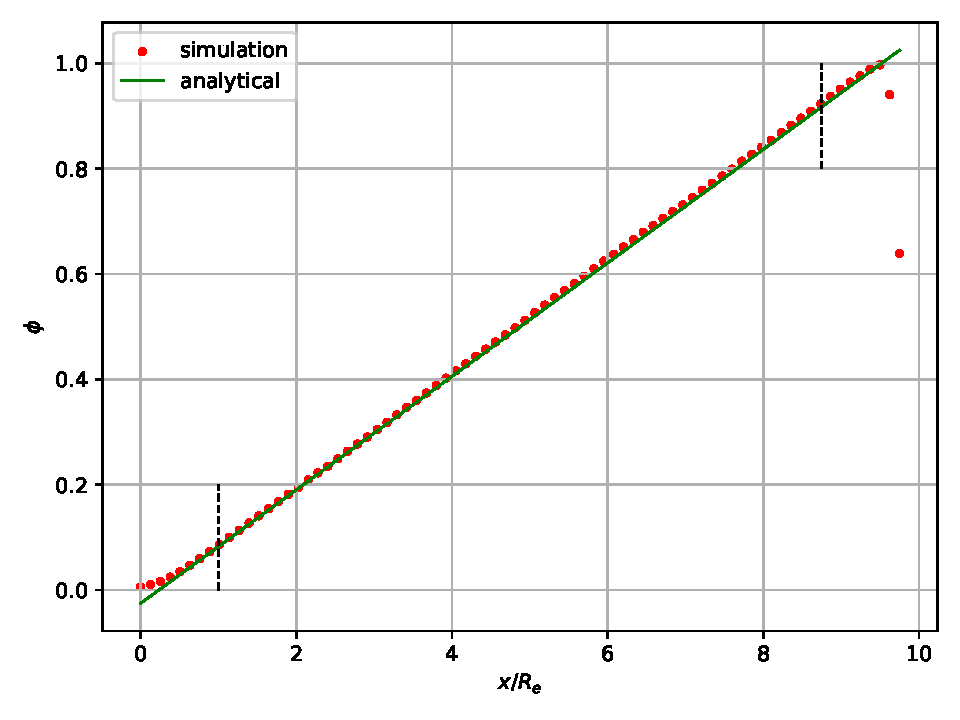
\includegraphics[width=0.6\linewidth]{figures/density_coll_diff.pdf}
  \caption{Steady-state density profile for $r=1.0$ averaged over $y$ and $z\,$. The analytical curve corresponds to \eqref{eq:density_profile_ana}. The black lines mark the region that is estimated to be affected by boundary effects.}
  \label{fig:density_profile}
\end{figure}

Outside of the range of the boundary effects, the density profile is very well represented by a linear function. The chemical potential is obtained by taking the functional derivative $\frac{\delta F}{\delta\phi}$ of \eqref{eq:flory_fctl}. Since $\chi=0\,$, no phase separation occurs and the local density differences are entirely due to the dynamics. Assuming the WSL, the chemical potential becomes:


\begin{align}
  \frac{\mu R_e^3}{\sqrt{\bar N} k_BT}&=\ln\phi-\ln(1-\phi)-\frac{R_e^2}{18\phi(1-\phi)}\phi''\nonumber \\ &+\left[\frac{R_e^2(1-2\phi)}{36\phi^2(1-\phi)^2}\right]\phi'^2\,,
  \label{eq:mu_flory}
\end{align}

where the dashes denote derivatives with respect to $x\,.$ The resulting chemical potential profile is shown in Figure \ref{fig:chemical_potential}.



\begin{figure}[h]
  \centering
  \begin{subfigure}[b]{0.45\textwidth}
      \centering
      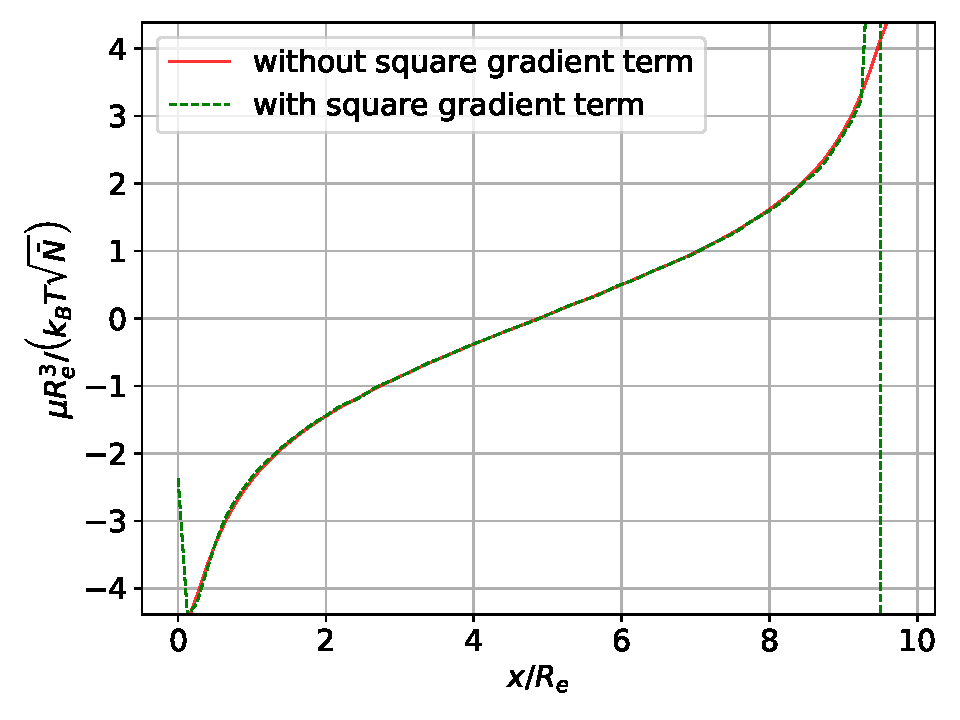
\includegraphics[width=\textwidth]{figures/mu_coll_diff.pdf}
      \caption{}
      \label{fig:chemical_potential}
  \end{subfigure}
    \hfill
  \begin{subfigure}[b]{0.45\textwidth}
      \centering
      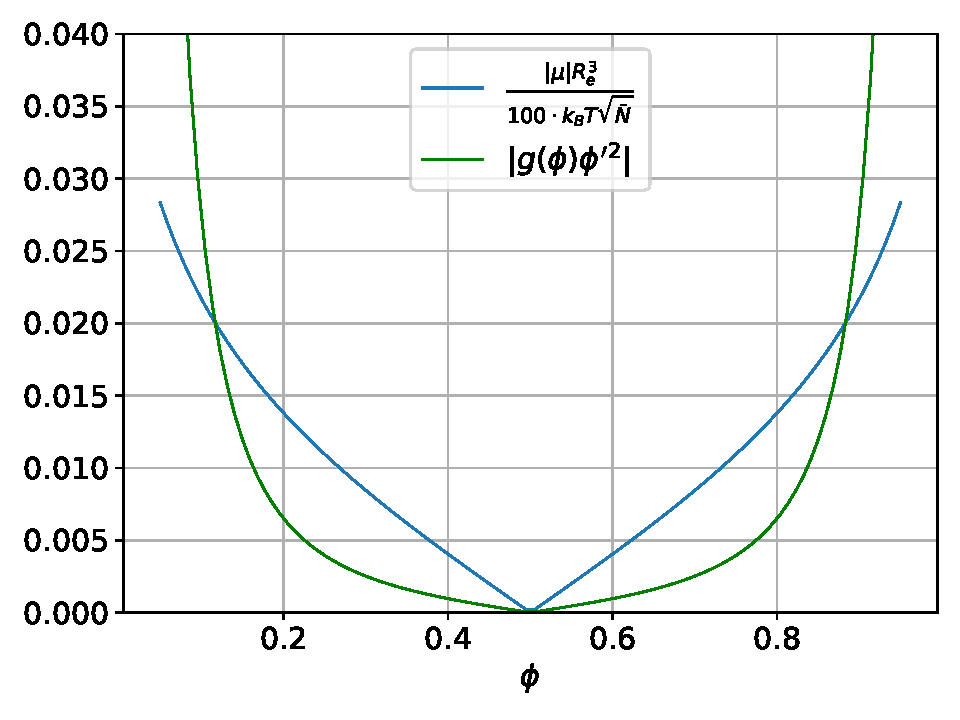
\includegraphics[width=\textwidth]{figures/squaregradient_contribution.pdf}
      \caption{}
      \label{fig:gradmu_fft}
  \end{subfigure}
     \caption{(a) Steady-state chemical potential profile obtained from \eqref{eq:mu_flory} for $r=1.0\,,$ averaged over $y$ and $z\,.$ (b) $g(\phi)\phi'^2\equiv R_e^2(1-2\phi)\phi'^2/[36\phi^2(1-\phi)^2]$ and absolute value of chemical potential $|\mu|R_e^3/(100\cdot k_BT\sqrt{\bar{N}})\,.$ In the discussed case, $\phi'\approx 0.1\,.$ }
     \label{fig:squaregradient_contribution}
\end{figure}


Evidently, the contribution of the terms involving spatial derivatives of the density to the total chemical potential is negligible, except in a very small region close to the walls. The linearity of the density profile already implies $\phi''=0$ and Figure \ref{fig:squaregradient_contribution} shows that the term proportional to $\phi'^2$ accounts for less than one percent of the total chemical potential for $0.12\lesssim\phi\lesssim 0.88\,,$ which roughly corresponds to the region in Figure \ref{fig:density_profile} that is assumed to be unaffected by boundary effects. In the subsequent discussion, the terms in \eqref{eq:mu_flory} containing spatial derivatives of $\phi$ will be neglected. This approximation improves further as the simulation box becomes infinitely long and $\phi'\rightarrow 0\,.$ However, for more complex density profiles, the contribution is of course not negligible.

With \eqref{eq:current_local} and \eqref{eq:mu_flory}, neglecting the terms arising from the square gradient, the current becomes:


\begin{align}
  J=-D\sqrt{\bar N}R_e^{-3}\phi'\,,
  \label{eq:current_a}
\end{align}


Together with \eqref{eq:conti}, this gives the standard diffusion equation:
\begin{align}
  \frac{\partial\phi(\mathbf r, t)}{\partial t}-D \phi''=0\,.
  \label{eq:diffusion}
\end{align}

where $D$ is obtained from \eqref{eq:einstein_relation}. In the steady state, this simply yields $\phi''=0\,,$ so a linear density profile is obtained, as expected. From \eqref{eq:current_a} and the condition that $\phi(L_x/2)=1/2\,,$ which follows from the symmetry of the conversion rates, the density profile becomes:

\begin{align}
  \phi(x)=\frac{JR_e^3}{D\sqrt{\bar{N}}}\left(\frac{L_x}{2}-x\right) + \frac{1}{2}\,,
  \label{eq:density_profile_ana}
\end{align}


To verify \eqref{eq:onsager}, the Onsager coefficient may also be obtained directly from the simulation results using \eqref{eq:current_local}. Again assuming local coupling and making use of \eqref{eq:mu_flory}, while neglecting the terms arising from the square gradient, one obtains:

\begin{align}
  \Lambda=-\frac{JR_e^3}{\sqrt{\bar N}\phi'}\phi(1-\phi).
  \label{eq:onsager_num}
\end{align}

The resulting Onsager coefficient is plotted in Figure \ref{fig:onsager_coeff}.

\begin{figure}[h]
  \centering
  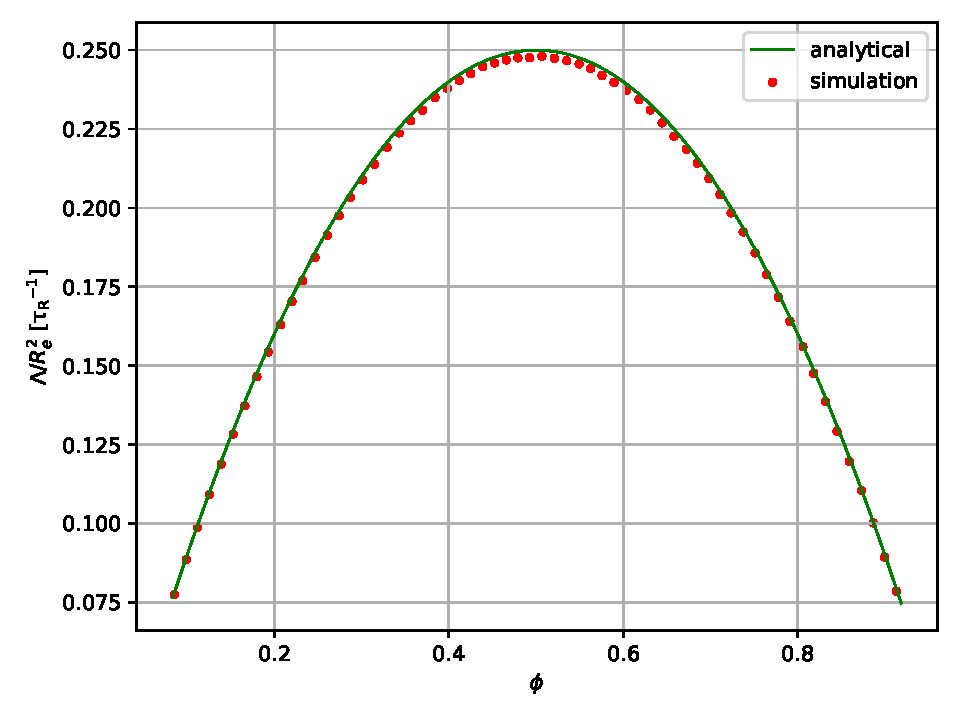
\includegraphics[width=0.6\linewidth]{figures/onsager_coll_diff.pdf}
  \caption{Onsager coefficient $\Lambda$ as a function of $\phi$. The analytical curve is obtained from \eqref{eq:onsager} and \eqref{eq:density_profile_ana}, the numerical curve from \eqref{eq:onsager_num} and the density profile in \ref{fig:density_profile}, where $\phi'$ is obtained from a linear fit. Only data points measured at a distance greater than $R_e$ from the walls are used. The diffusion constant $D$ and the current $J$ are both obtained from the simulation.}
  \label{fig:onsager_coeff}
\end{figure}

The Onsager coefficients obtained from \eqref{eq:onsager} and \eqref{eq:onsager_num} are in excellent agreement, which hints that the theoretical derivations are consistent with the simulation results. 
Specifically, the assumptions of incompressibility and local coupling of the current to the chemical potential are justified and the linear density profile observed in Figure \ref{fig:density_profile} is explained.


\chapter{External-field-driven flow}

One of the simplest ways to implement time-dependent boundary conditions in \ac{SOMA} is to apply time-dependent external fields that are only nonzero close to the boundaries and have the form:

\begin{align}
    E_i(\mathbf{r},t)=f_i(\mathbf r,t)\phi_i({\mathbf r,t})\,,
\end{align}

where $i=\mathrm A,\mathrm B$ denotes the monomer types. In this section, layers of lamellar diblock-copolymers are moved at constant speed $v$ perpendicular to their orientation using spatially periodic external fields close to the boundaries. In a system that moves along with the external field, each monomer experiences a friction force $\zeta v$ in the opposite direction, where $\zeta$ is obtained from \eqref{eq:d_rouse}. The degree of deformation depends on the P\'eclet number $P_e\equiv vR_e/D\,.$ For large values $P_e\approx 1\,,$ the chains cannot keep up with the external field movement and the lamellae break. For small $P_e\approx0\,,$ they have enough time to fully relax to the undeformed shape. In this section, an intermediate regime is investigated to obtain the bending modulus $K\,.$ 

\section{Reference system}
A system of $n=750$ symmetric diblock-copolymers with $N_A=N_B=N/2=16$ and $\chi N=20$ is used. The box dimensions are $L_x\times L_y\times L_z=2.5\times2.82\times1\,R_e^3\,,$ which corresponds to $\sqrt{\bar{N}}=106\,.$ The spatial discretizations are $\Delta x=1/16\,R_e\,,$ $\Delta y=47/800\,R_e$ and $\Delta z=1\,R_e\,.$ To generate the initial lamellar structure, external fields are applied, as shown in Figure \ref{fig:fext}. The interlayer spacing of $d=1.41\,R_e$ was found to be stable over the duration of the simulations, but it does not correspond to the equilibrium spacing.

Subsequently, the external fields are switched off everywhere except at a distance less than $b=0.5\,R_e$ from the boundaries in the $x$-direction, so the length of the part of the lamellae that is not supported by the external fields is $L=1.5\,R_e$. Every $\Delta t$ MCS, the fields are moved by a distance of $\Delta y$ in the $y$-direction, so the velocity is $v=47R_e/(800\Delta t)\,.$ The external fields balance the friction forces at the boundaries and therefore act as bearings for the lamellae. The diffusion constant $D$ is obtained from \eqref{eq:einstein_relation}, where $g_3(t)$ is measured in a system without external fields and $\chi N=0\,.$

\begin{figure}[h]
    \centering
    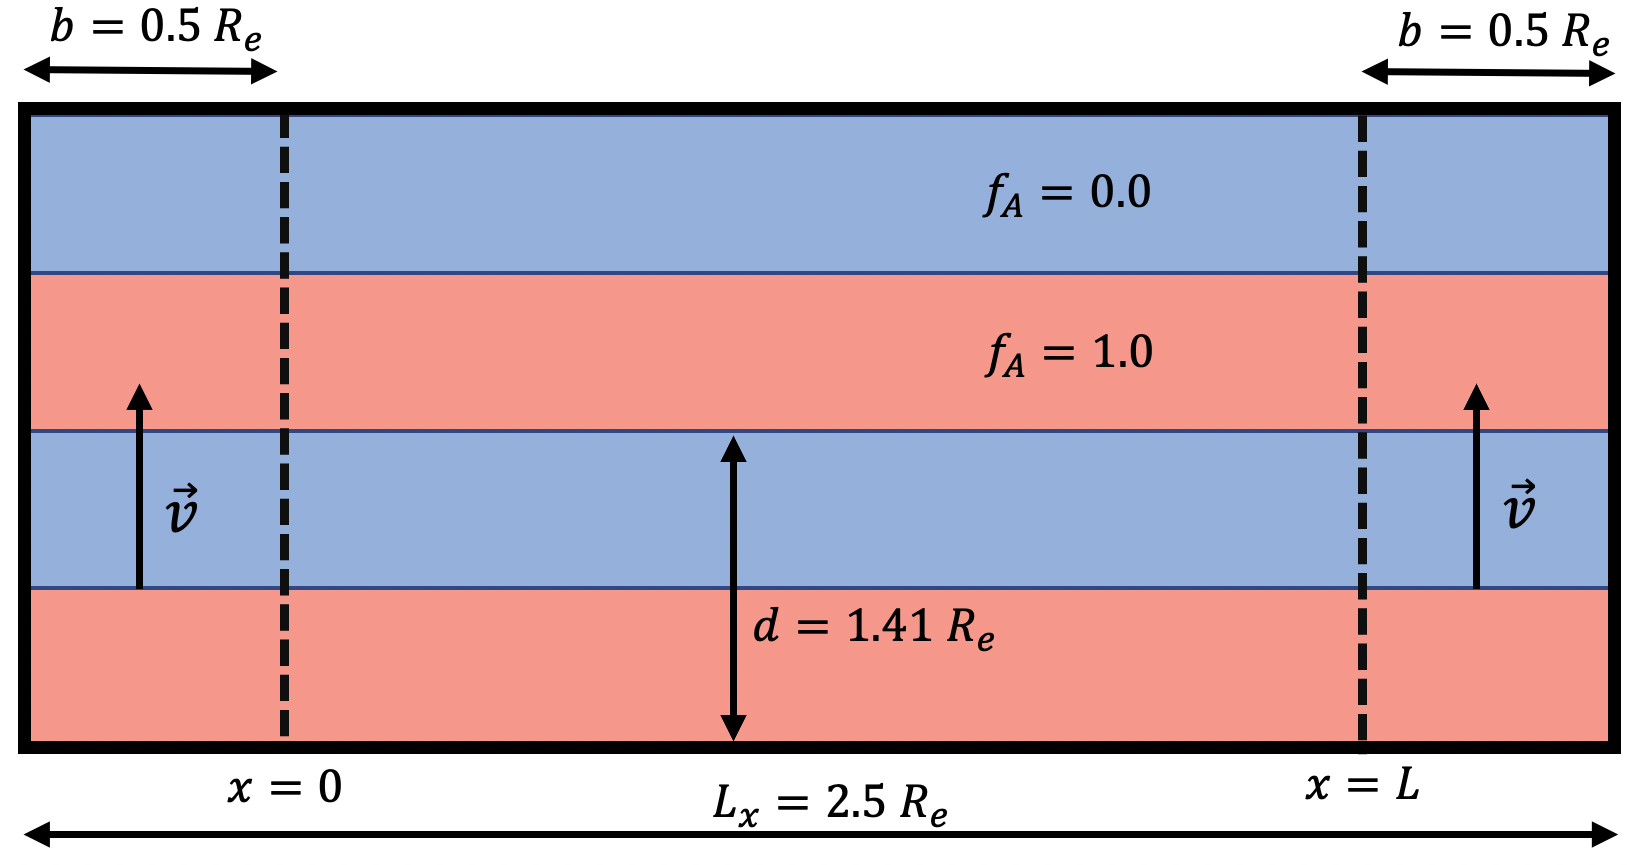
\includegraphics[width=0.6\linewidth]{figures/fext.png}
    \caption{Sketch of the external field $f_\text A(\mathbf r,0)\,.$ Red domains correspond to $f_\text A=1.0\,,$ blue domains to $f_\text A=0.0\,.$ $f_\text B(\mathbf r,0)$ is exactly complementary. Within the region bounded by the dotted lines, the external fields are switched off after the initial lamella structure has been generated.}
    \label{fig:fext}
\end{figure}


\section{Bending modulus}
For small deformations, in the \ac{SSL}, the free energy of a bent lamella is \cite{wang94}:

\begin{align}
    F&=\int d\mathbf r\left\{f_0+\frac{1}{2}K \left(\partial_x^2 u\right)^2\right\}\,,\\
    &\approx dL_z\int dx\left\{f_0+\frac{1}{2}K \left(\partial_x^2 u\right)^2\right\}\nonumber\\
    &\equiv dL_z\int dxf(u,u'')\,.
    \label{eq:F_bend}
\end{align}

where $f_0$ is the free energy per unit volume of the unbent lamella, $K$ is the bending modulus and $u\equiv u(x)$ is the deformation profile of the A-B-interface. For the integration over $y$ and $z\,,$ the change of volume was neglected. The friction force density is $q_{fric}=N\sqrt{\bar N}\zeta P_eD/R_e^4\,.$ In the steady-state, it is balanced by a force density given by the  functional derivative $\delta F/\delta u\,$:

\begin{align}
    \frac{\delta F}{\delta u}&=q_{fric}=\frac{\partial^2}{\partial x^2}\frac{\partial f}{\partial u''} \nonumber \\
    \implies K\frac{\partial^4u}{\partial x^4}&=N\sqrt{\bar N}\zeta\frac{P_eD}{R_e^4} \,.
\end{align}


With the boundary conditions $u(0)=u(L)=0$ and $u''(0)=u''(L)=0\,,$ one obtains:
\begin{align}
    u(x)=\frac{N\sqrt{\bar N}\zeta P_e Dx}{24KR_e^4}(L^3-2L^2x+x^3)\,,
    \label{eq:deflection}
\end{align}
in analogy to a beam bending under a uniform load in the Euler-Bernoulli theory. The resulting lamella profile for $P_e=0.24$ is shown in Figure \ref{fig:lamella_bent}. The fit is in excellent agreement with the simulation data. 



\begin{figure}[h]
  \centering
  \begin{subfigure}[b]{0.45\textwidth}
      \centering
      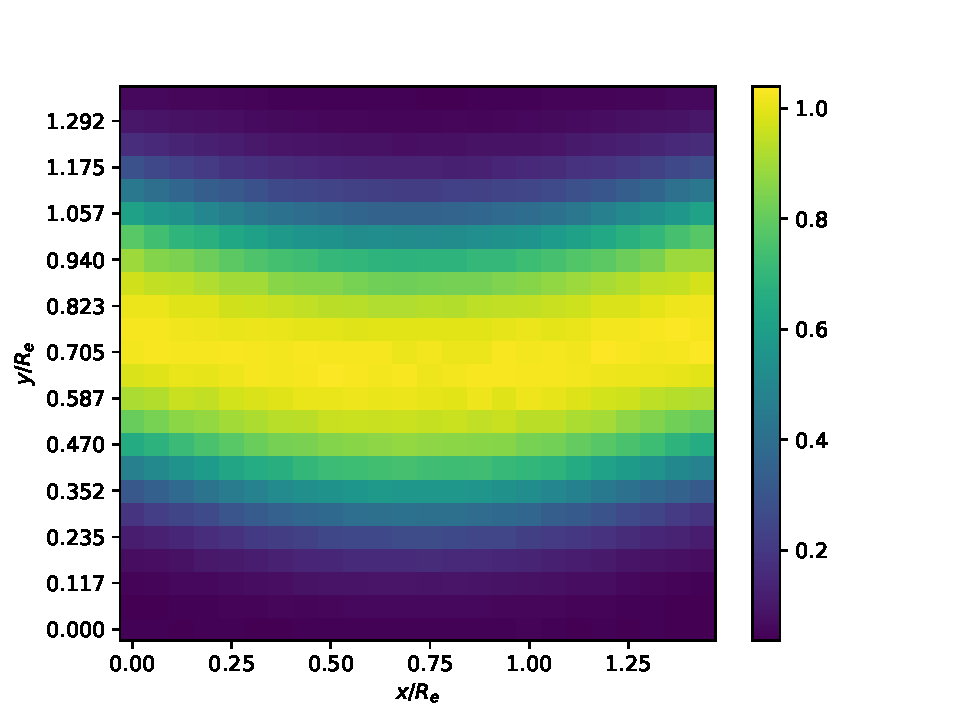
\includegraphics[width=\textwidth]{figures/heatmap_t2000.pdf}
      \caption{}
      \label{fig:lamella_heatmap}
  \end{subfigure}
    \hfill
  \begin{subfigure}[b]{0.45\textwidth}
      \centering
      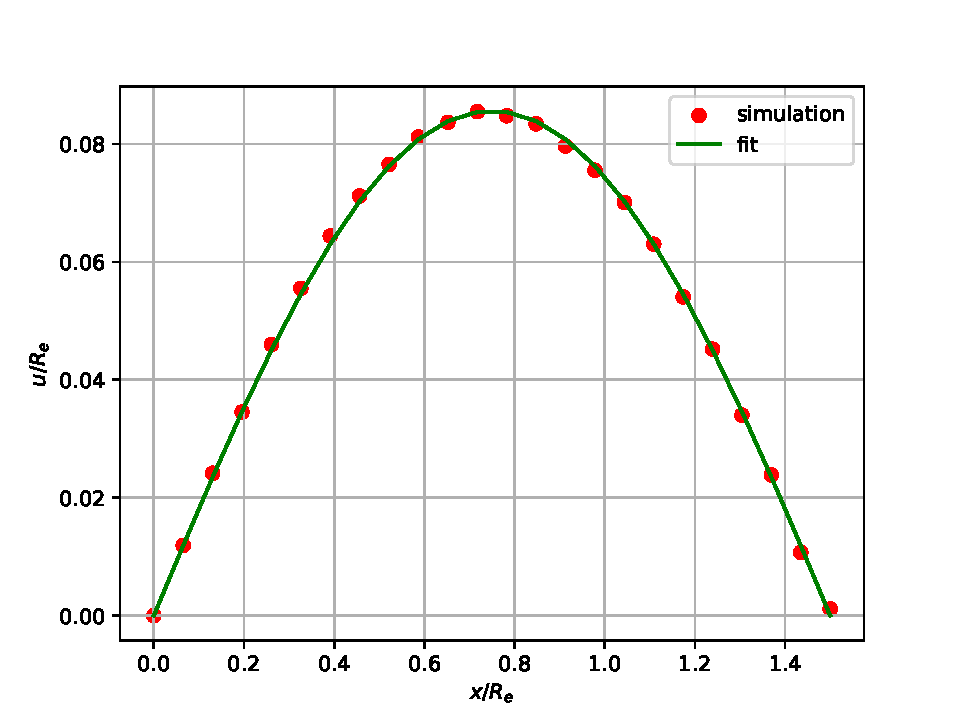
\includegraphics[width=\textwidth]{figures/lamella_profile_t2000.pdf}
      \caption{}
      \label{fig:lamella_deflection}
  \end{subfigure}
     \caption{(a) Heatmap of the steady-state lamella profile in the reference frame that moves with the external field, averaged over all lamellae. (b) Lamella center of mass curve for $P_e=0.34\,$. The fit corresponds to \eqref{eq:deflection}.}
     \label{fig:lamella_bent}
\end{figure}


The maximum deformation is:
\begin{align}
    u_{max}=u(L/2)=\frac{5N\sqrt{\bar N}\zeta P_e DL^4}{384KR_e^4}\,.
    \label{eq:umax}
\end{align}

To obtain the bending modulus, $u_{max}$ is measured for various values of $P_e\,$, this is shown in Figure \ref{fig:stress_strain}.

\begin{figure}[h]
    \centering
    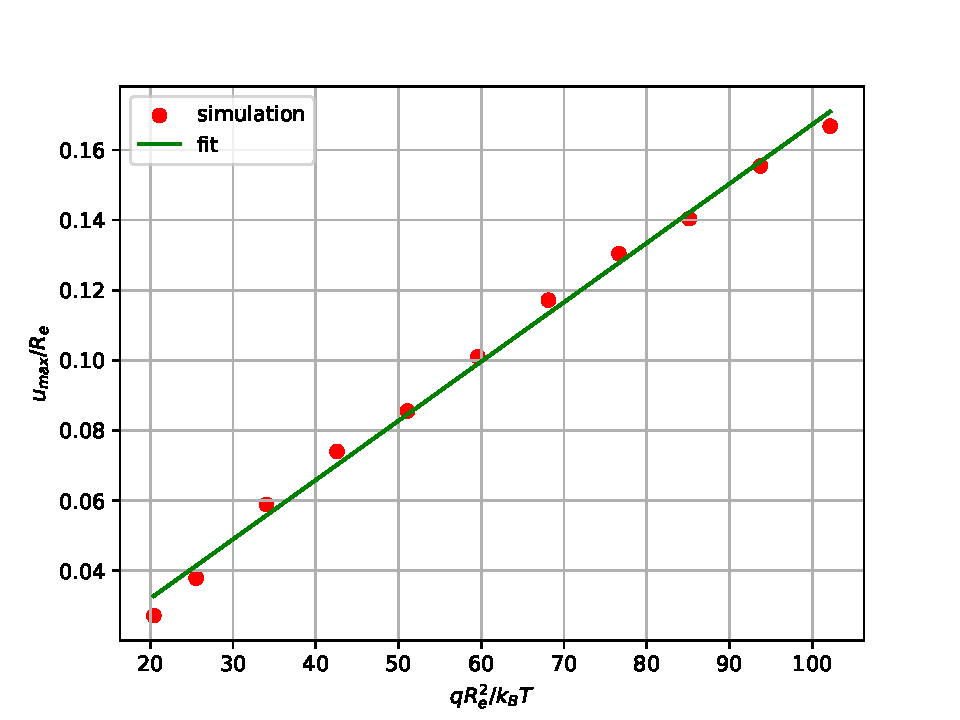
\includegraphics[width=0.6\linewidth]{figures/stress_strain_plot.pdf}
    \caption{Maximum deflection  $u_{max}$ as a function of the P\'eclet number $P_e\,.$ The fit corresponds to \eqref{eq:umax}.}
    \label{fig:stress_strain}
\end{figure}


From $\eqref{eq:umax}\,,$ one obtains $K=19.98\,k_BT/R_e\,.$ Alternatively, $K$ may also be obtained from exact \ac{SCFT}. For this, the free energy of bending is computed for a sinusoidal deformation $u(x)=a\sin2\pi x/L\,,$ as shown in Figure \ref{fig:bend_scft}. From \eqref{eq:F_bend}, the total free energy may be calculated as:

\begin{align}
    F&=dL_z\int dx\left\{f_0+\frac{1}{2}Ka^2\left(\frac{2\pi}{L}\right)^4\sin\left(\frac{2\pi}{L}x\right)^2\right\}\nonumber\\
    &\approx dLL_zf_0+dL_z\frac{4\pi^4a^2}{L^3}K\,.
    \label{eq:f_scft_1}
\end{align}

On the other hand, the total free energy may be obtained by integrating over the free energy density:
\begin{align}
    F&=\int d\mathbf r(f_0+f_b)\nonumber\\
    &\approx dLL_z(f_0+f_b)\nonumber \\
    &=dLL_z\frac{\sqrt{\bar N}}{R_e^3}(\tilde f_0+\tilde f_b)\,,
    \label{eq:f_scft_2}
\end{align}

where $\tilde f_0=4.0337\,k_BT$ is the free energy per chain of the undeformed lamella and $\tilde f_b=0.79278\,k_BT(a/R_e)^2$ is the free energy per chain due to the deformation. Comparing \eqref{eq:f_scft_1} and \eqref{eq:f_scft_2}, the bending modulus reads:

\begin{align}
    K_\text{SCFT}=\frac{\tilde f_b\sqrt{\bar N}}{4a^2\pi^4}R_e^{-3}L^4\,.
\end{align}

The result is $K_\text{SCFT}=17.47\,k_BT/R_e\,,$ which is slightly smaller than the simulation result. 

% \begin{itemize}
%     \item The following discussion can probably be omitted
% \end{itemize}

% In equilibrium, it may also be obtained directly from the simulation parameters \cite{wang94}:


% \begin{align}
%     K=\frac{3}{16}\left(\frac{12}{\pi^2}\right)^{1/3}\left(\frac{\gamma}{k_BT}\right)^{4/3}\bar N^{-1/6}R_e^{5/3}k_BT\,,
%     \label{eq:k_ana}
% \end{align}

% where $\gamma$ is the interfacial tension. In the strong segregation limit, it reads (\textbf{Hier evtl Faktor 3 wegen 3 Grenzflaechen?})\cite{semenov1996}:

% \begin{align}
%     \frac{\gamma R_e^2}{\sqrt{\bar N}k_BT}=\sqrt{\frac{\chi N}{6}}\left(1-\frac{4\ln 2}{\chi N}\right)\,.
% \end{align}


% The result is $K=38.94\,k_BT/R_e\,,$ in excellent agreement with the simulation results. However, it should be noted that $\eqref{eq:k_ana}$ is derived from the equilibrium spacing $d_0\,.$ For $\chi N=20\,,$ \cite{wang94} predicts $d_0=1.24\,R_e\,,$ which is too small (\textbf{Need some reference value here to cite}). This is likely to indicate that the strong segregation is not fully reached at $\chi N=20\,.$ Nevertheless, the results might suggest that the bending modulus $K$ only weakly depends on the monolayer tickness.


\begin{figure}[h]
    \centering
    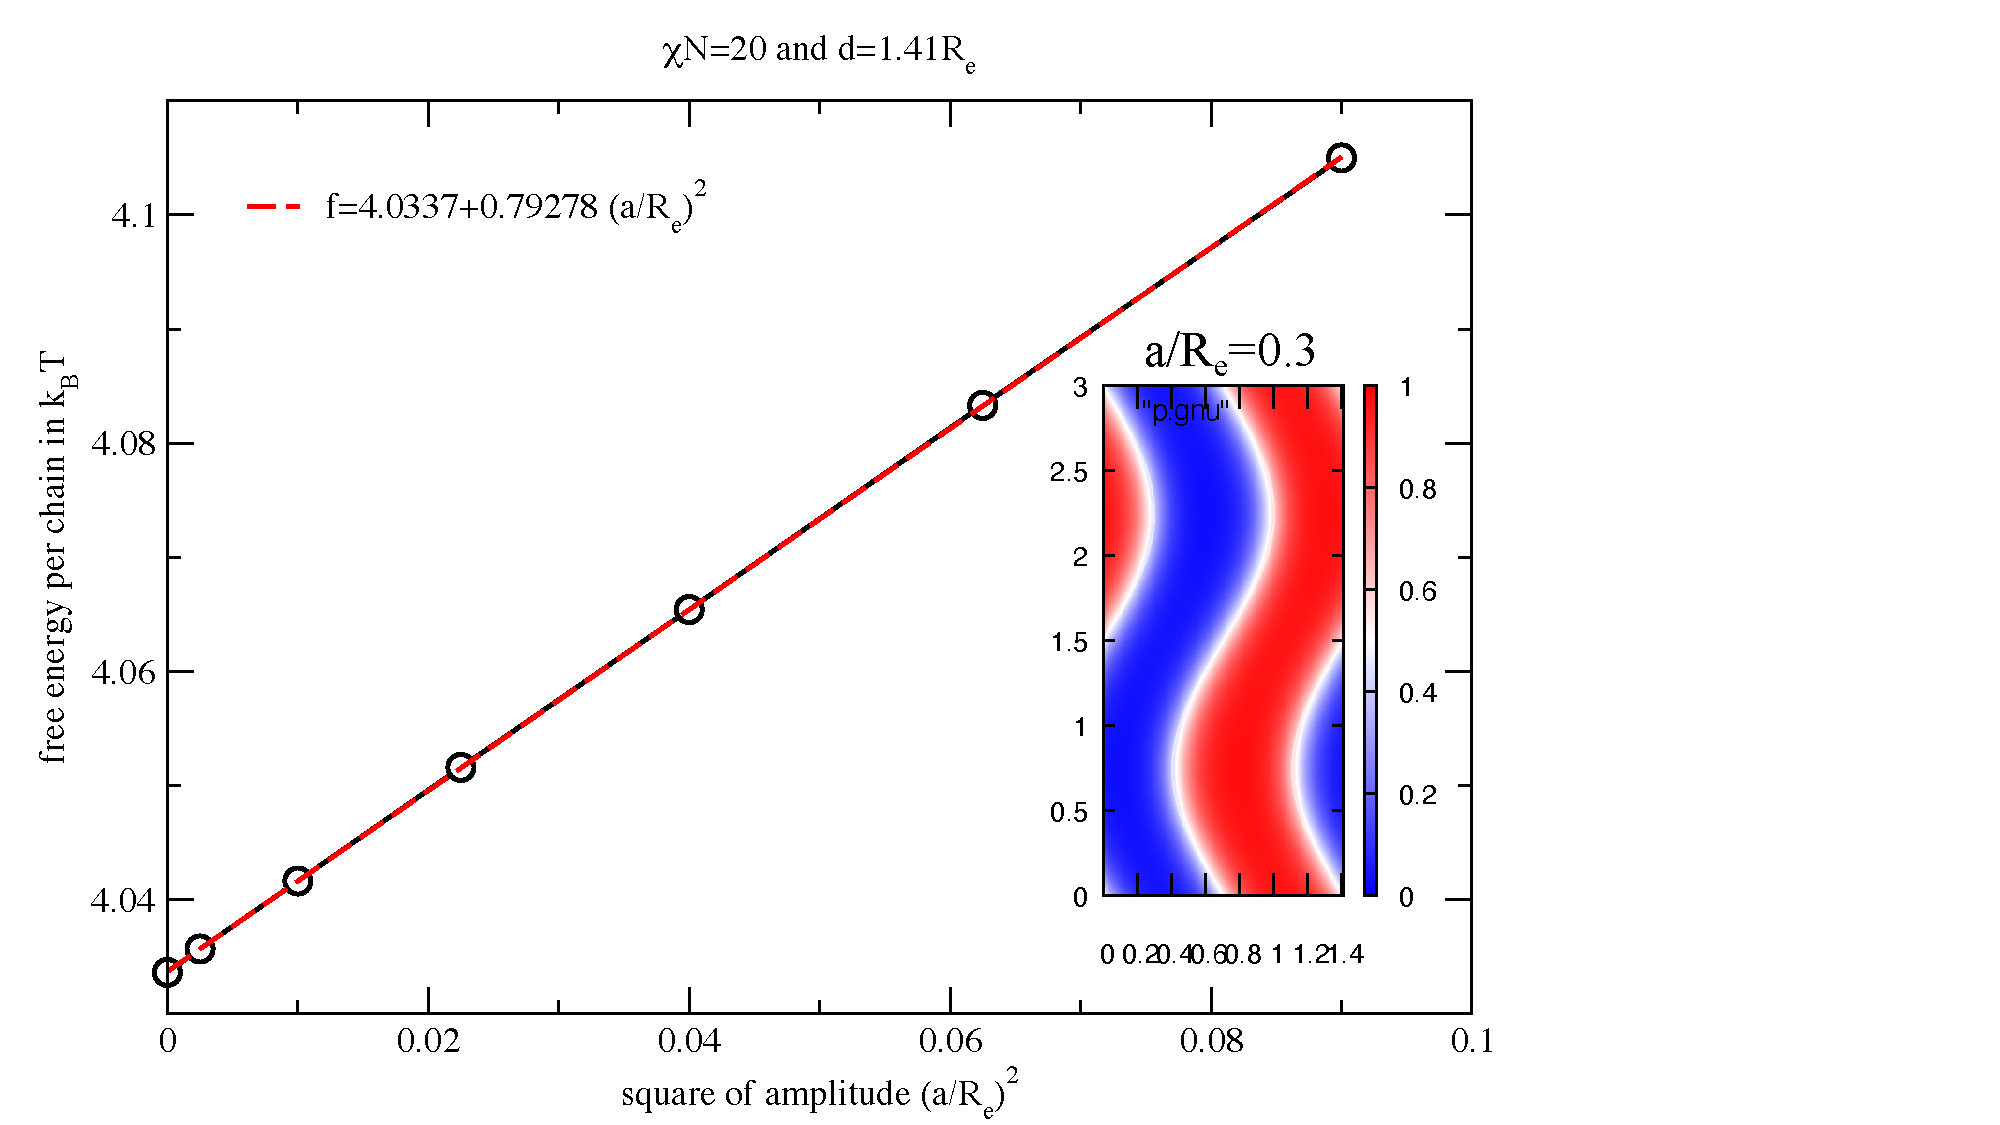
\includegraphics[width=0.6\linewidth]{figures/bend_scft.pdf}
    \caption{Free energy per chain as a function of the square of the amplitude from exact \ac{SCFT} calculations. The inset shows the lamella cross-section for $a/R_e=0.3\,.$}
    \label{fig:bend_scft}
\end{figure}

\chapter{Polymer-type-conversion-based target density}
\section{Formulation of the problem}
We now want to take a step towards simulating the setting depicted in Figure \ref{fig:continuum_section}. For this, we define the composition of bead-type $\alpha$ in cell $c$ as:

\begin{align}
    \tilde\phi_\alpha(c)=\frac{\hat\phi_\alpha(c)}{\sum_{i=1}^{n_t}\hat\phi_i(c)}=\frac{n_\alpha(c)}{\sum_{i=1}^{n_t}n_i(c)}\,,
\end{align}



where $n_i(c)$ is the number of beads of type $i$ in cell $c\,.$ To dictate the composition in specific cells, target values $\tilde\phi_{\alpha,T}(c)$ are defined, with $\tilde\phi_{\alpha,T}(c)<0$ $\forall\alpha$ for cells in which no target composition is desired. In the following, the cells $c$ for which $\tilde\phi_{\alpha,T}(c)\ge 0$ $\forall\alpha$ are called \enquote{target cells}. Mixed cells with $\tilde\phi_{\alpha,T}(c)\ge 0$ for some $\alpha$ and $\tilde\phi_{\alpha,T}(c)<0$ for other $\alpha$ are not allowed and target cells must fulfill the condition $\sum_\alpha\tilde\phi_{\alpha,T}(c)=1\, .$  (\textbf{Write a test to ensure this is true!}). The total number of target cells is denoted $n_T\,.$ Instead of using external fields, like in the previous section, the goal is to reach the target density by converting macromolecule types, see chapter \ref{chap:colldiff}. For now, only conversions between macromolecules with the same bond topology are considered. Due to the chain connectivity, this leads to a complex optimization problem for the polymer type configurations, which aims to minimise the following loss function:

\begin{align}
    L[\{\tilde\phi_i\}]=\sum_{\alpha=0}^{n_t}\sum_{c\in \{\text{cells}\}}\theta(\tilde{\phi}_{\alpha,T}(c))\left(\tilde{\phi}_\alpha(c)-\tilde{\phi}_{\alpha,T}(c)\right)^2\,,
    \label{eq:lossfunction}
\end{align}

where $\theta(\tilde{\phi}_{\alpha,T}(c))=1$ if $\tilde{\phi}_{\alpha,T}(c)\ge 0$ and $\theta(\tilde{\phi}_{\alpha,T}(c))=0$ otherwise. Let $n_f$ be the number of polymers that have at least one monomer in a target cell $c\,.$ In the following, these polymers are called \enquote{flippable polymers}. To minimise $\eqref{eq:lossfunction}$, one must first define the notion of a neighbouring solution. If $\{\beta_1,\dots,\beta_j,\dots\beta_{n_f}\}$ is the current configuration of polymer types, then we define a neighbouring solution as $\{\beta_1,\dots,\beta^*_j,\dots\beta_{n_f}\}\,,$ where the type of the $j$th polymer has been changed from $\beta_j$ to $\beta_j^*$ and every other polymer type is unchanged. In the following, this rule to generate a neighbouring solution is called a \enquote{flip}. The flippable polymers are identified and saved to a list by algorithm \ref{alg:get_flip_candidates}. $n_f$ is not constant and must be determined during runtime. The target cells in which a flippable polymer $j$ has monomers are saved to an $n_f\times N$ matrix $q_{jk}\,.$ The number of target cells $n_{cells,j}\,,$ over which a flippable polymer $j$ extends, varies, and is bounded by $N\,,$ this is incorporated by setting $q_{jk}<0$ for $k\ge n_{cells,j}\,.$ Let $n_{j\beta\alpha k}$ be the $n_f\times m_t\times n_t\times N$ matrix that holds the number of monomers of type $\alpha$ that flippable polymer $j$ has in target cell $q_{jk}$ if it has the molecule type $\beta\,,$ where $n_{j\beta\alpha k}=0$ for $k\ge n_{cells,j}\,.$ After the flip $\beta_j\rightarrow \beta_j^*$ of an arbitrary, flippable polymer $j\,,$ the value of the loss function is updated according to:

\begin{align}
    L^*_{\beta_j\rightarrow\beta_j^*}[\{\tilde\phi_i\}] &= L[\{\tilde\phi_i\}] 
    - \sum_{\alpha=0}^{n_t}\sum_{k=0}^{n_{cells,j}-1}  \left(\tilde{\phi}_\alpha(q_{jk})-\tilde{\phi}_{\alpha,T}(q_{jk})\right)^2\nonumber \\
    & \quad + \sum_{\alpha=0}^{n_t}\sum_{k=0}^{n_{cells,j}-1}  \left(\tilde{\phi}_\alpha(q_{jk})+\Delta\tilde\phi_{ j\alpha k}(\beta\rightarrow\beta^*)-\tilde{\phi}_{\alpha,T}(q_{jk})\right)^2\nonumber \\
    &= L[\{\tilde\phi_i\}] 
    + \sum_{\alpha=0}^{n_t}\sum_{k=0}^{n_{cells,j}-1}  \biggl\{\Delta\tilde\phi^2_{ j\alpha k}(\beta\rightarrow\beta^*) \nonumber\\
    &\quad + 2\Delta\tilde\phi_{ j\alpha k}(\beta\rightarrow\beta^*)\left(\tilde\phi_{\alpha}(q_{jk})-\tilde\phi_{\alpha,T}(q_{jk})\right)\biggr\}
\end{align}

where $\Delta\tilde\phi_{ j\alpha k}(\beta\rightarrow\beta^*)\equiv\frac{n_{j\beta_j^*\alpha k}-n_{j\beta_j\alpha k}}{\sum_{i=1}^{n_t}n_i(c)}$ is the change in the composition of type $\alpha$ in cell $q_{jk}$ due to the flip $\beta_j\rightarrow\beta_j^*\,$. Thus, for an efficient implementation of an optimization algorithm, the matrices $q_{jk}$ and $n_{j\beta\alpha k}$ have to be determined first. How this is done with the memory structure used in \ac{SOMA} is explained in algorithms \ref{alg:get_cell_indices} and \ref{alg:get_cell_numbers}. 

\section{Steepest descent}

In the \ac{SD} algorithm, flippable polymers are selected at random and flipped to a random target type. The flip is only accepted if it decreases the loss function. $n_{acc}$ counts the number of accepted flips. Every $n_f$ flips, the acceptance rate $r=n_{acc}/n_f$ is calculated and $n_{acc}$ is reset to zero until the convergence criterion $r=0$ is fulfilled. Then, each flippable polymer is given one more chance to be flipped. Since this algorithm is only guaranteed to find a local minimum, more sophisticated optimization alogrithms may need to be employed.

\section{Simulated annealing}

If neighbouring solutions are generated by the flip of a single polymer type, \eqref{eq:lossfunction} is not a convex function of the polymer type configurations, this is discussed in Figure \ref{fig:loss} in the appendix. Therefore, a simple \ac{SD} algorithm, as discussed in the previous section, might fail at finding the global minimum. To tackle these kind of combinatorial optimization problems, the probabilistic \ac{SA} technique \cite{simulated_annealing} is frequently used. In this heuristic algorithm, a parameter $T$ is introduced in analogy to temperature in statistical mechanics. Starting from a predefined temperature $T_0\,,$ an initial guess $S$ for the solution and a loss function $L\,$, a neighbouring solution $S^*$ is generated by a specific rule and accepted with a probability given by the Metropolis-Hastings criterion, similarly to \eqref{eq:metropolis_mc}:

\begin{align}
    p(S\rightarrow S^*)=\min\left\{1\,,\exp\left(-\frac{L(S^*)-L(S)}{T}\right)\right\}\,.
\end{align}

Subsequently, the temperature is decreased by a predefined scheme and the procedure is repeated until a final temperature $T_f$ is reached. A slightly modified algorithm that generates multiple neighbouring solutions for each temperature $T$ is used in this thesis and explained in algorithm \ref{alg:sa} in the appendix.

\section{Comparison of algorithms}

In order to compare the performance of the two presented algorithms, several randomly generated initial configurations are optimized with lamellar  target densities. A binary blend of homopolymers with $N=32$ and $\sqrt{\bar N}=100$ is used. The box dimensions are $L_x\times L_y\times L_z=5\times1\times5\,R_e^3$ with $\Delta L=1/8\,R_e$ and hard, impenetrable  walls are applied at all boundaries. The target composition is defined directly behind the walls with a width of one grid point. The lamella periodictiy is characterized by a wave number $q$ and the deviation of the lamella composition from the homogeneous value is given by $\Delta\tilde\phi\,,$ so the target values are $0.5\pm\Delta\tilde\phi\,.$ A simple linear cooling schedule is employed for the \ac{SA} algorithm:

\begin{align}
    T_k=T_0-\alpha k\,.
\end{align}

Optimizations are performed on 50 different initial structures. The loss function is normalized by the number monomer types $n_t\,,$ the number of target cells $n_T$ and the natural density fluctuations $\sigma_0^2\,,$ which is calculated as $\sigma_0^2=1/\rho_0\Delta L^3\kappa$ in the mean field approximation \cite{Daoulas06}. The \ac{SA} algorithm is run after the \ac{SD} algorithm, so it starts from a local minimum of \eqref{eq:lossfunction}. The resulting optimized structures are shown in Figure \ref{fig:comparison_sd_sa} for different parameters. For $\Delta\tilde\phi=0.1$ and $qR_e/2\pi=0.8\,,$ the optimized composition profile matches the target profile very well. For $\Delta\tilde\phi=0.49\,,$ only an amplitude of about $0.35$ is reached. For  $qR_e/2\pi=4.0\,,$ which corresponds to the highest possible lamella frequency of the used grid discretization, the amplitude further decreases to to about $0.11\,.$ Interestingly, the composition profiles obtained from \ac{SD} and \ac{SA} are virtually the same. Figure \ref{fig:comparison_sd_sa} shows that the composition clearly drops after staying on a plateau given by the local minimum that it started from. The critical temperature $T^*$ of this drop depends on $q$ and $\Delta\tilde\phi\,.$ After the steep drop, the loss function reaches a plateau region again, which likely corresponds to the global minimum. The difference between the two plateau regions is very small. For $\Delta\tilde\phi=0.1\,,$ one obtains $\Delta L_{opt}/n_tn_T\sigma_0^2\approx 0.04\,.$ This value decreases even further as $\Delta\tilde\phi$ is increased, as shown in Figure \ref{fig:dl_dphi}. The acceptance rate does not display any particular change of course at the critical temperature $T^*\,.$ This shows that any local minima that the \ac{SD} algorithm may become trapped in are already close to the global minimum. Since the computational cost of the \ac{SA} algorithm outweighs the improvement in the loss function by far, it is concluded that the \ac{SD} algorithm is sufficient. 

\begin{figure}[htbp]
    \centering
    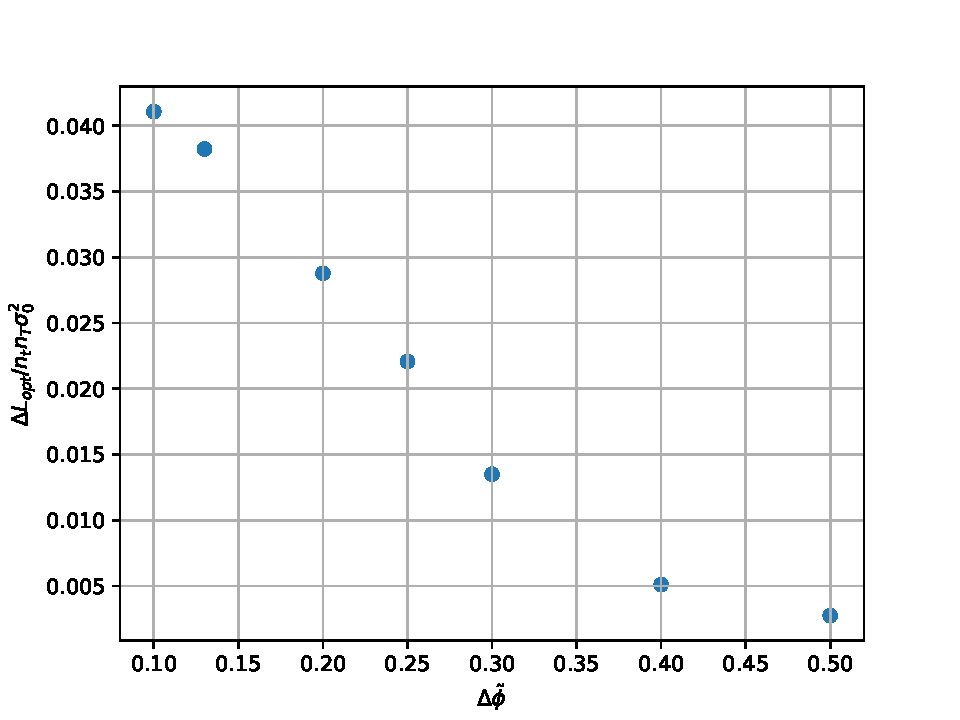
\includegraphics[width=0.7
    \linewidth]{figures/dL-dphi.pdf}
    \caption{Change of loss function after kink as a function of $\Delta\tilde\phi\,.$}
    \label{fig:dl_dphi}
\end{figure}



\begin{figure}[htbp]
    \centering
    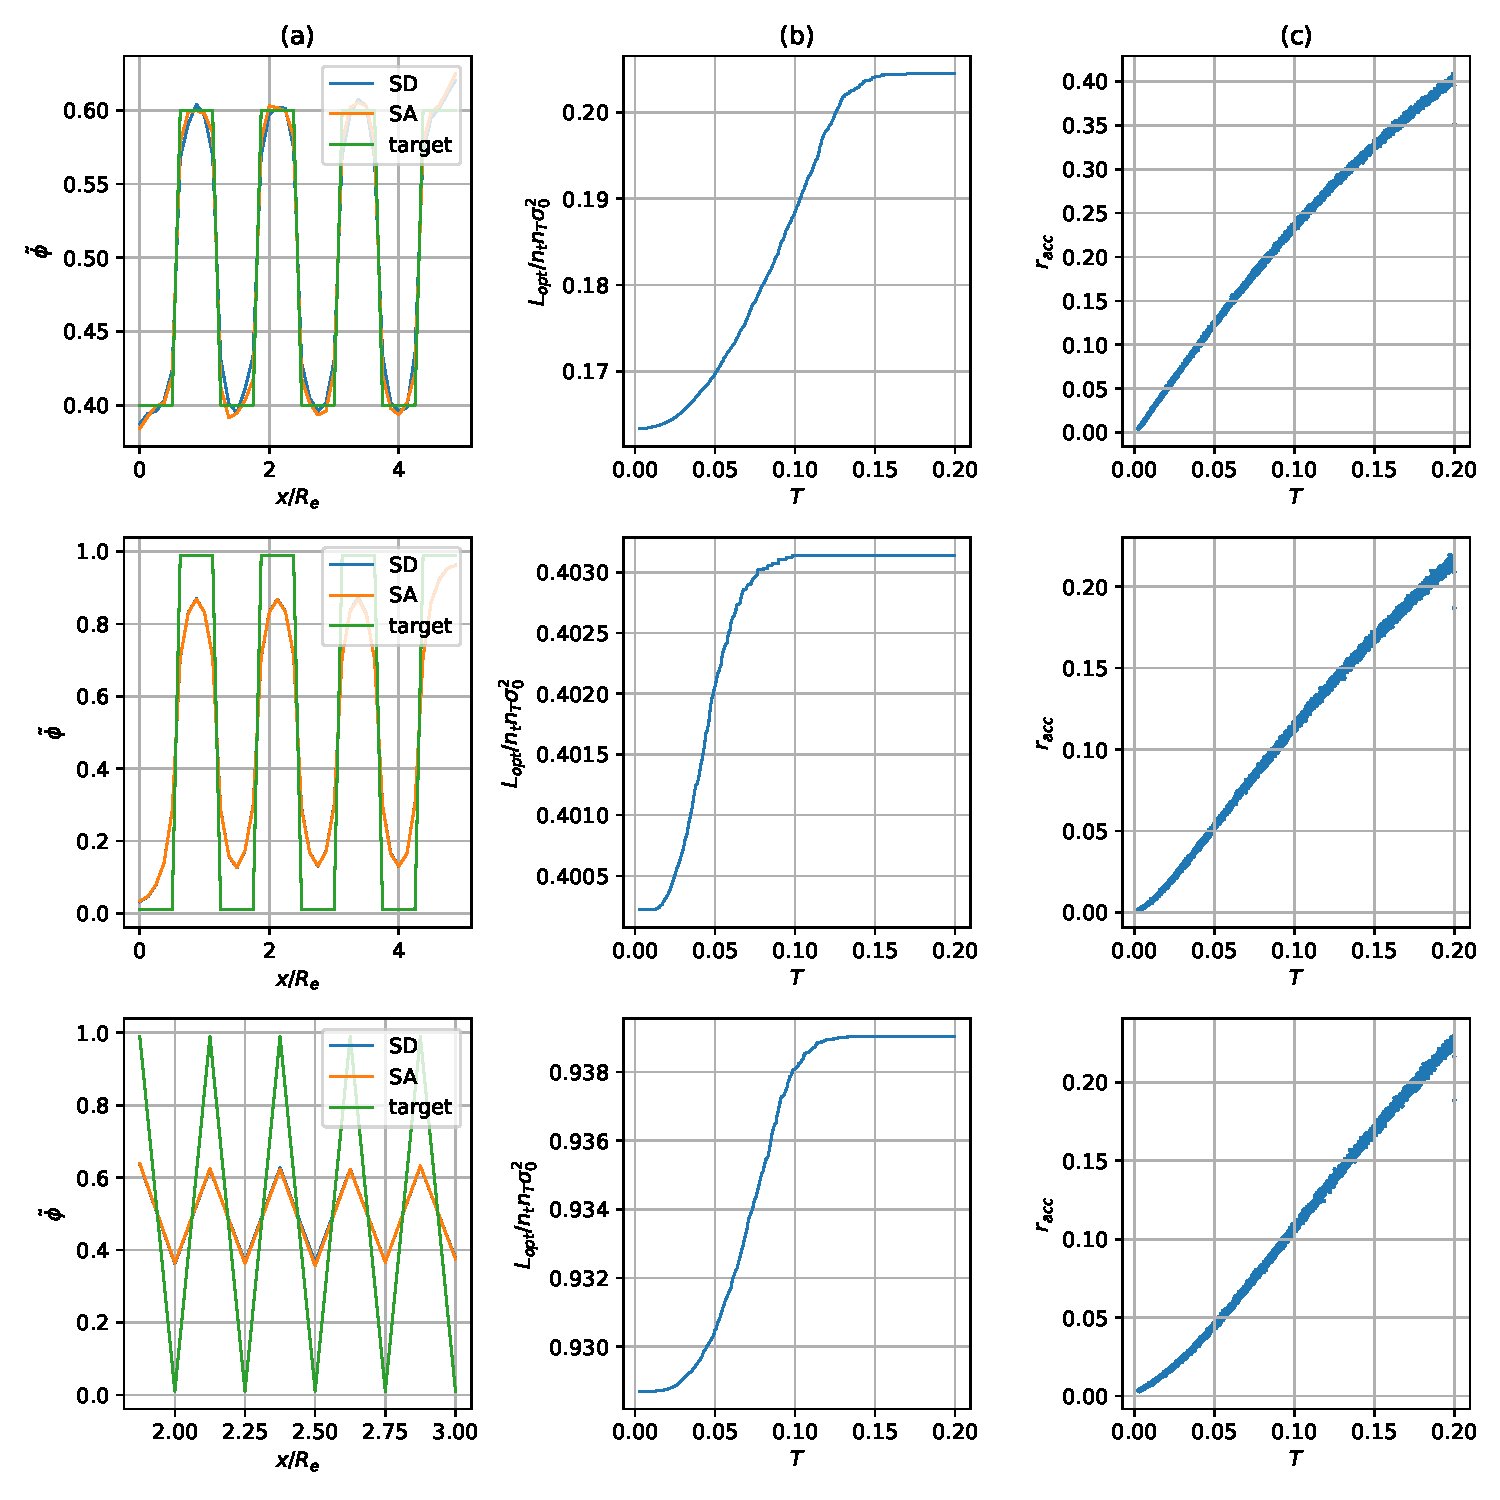
\includegraphics[width=\linewidth]{Thesis/figures/comparison_sd_sa.pdf}
    \caption{(a) Amplitude after optimization and target profile. (b) \ac{SA} optimum as a function of temperature. (c) Acceptance rate as a function of temperature. Top: $qR_e/2\pi=0.8\,,$ $\Delta\tilde\phi=0.1\,.$ Middle: $qR_e/2\pi=0.8\,,$ $\Delta\tilde\phi=0.49\,$ Bottom: $qR_e/2\pi=4.0\,,$ $\Delta\tilde\phi=0.49\,.$ For clarity, only a section of the $x$ axis is plotted for $qR_e/2\pi=4.0\,.$}
    \label{fig:comparison_sd_sa}
\end{figure}



% \subsection{Reference system}

% A system of $n=5000$ homopolymers with $N_A=N_B=N=32$ and $\chi N=0$ is used. The box dimensions are $L_x\times L_y\times L_z=5\times1\times5\,R_e^3\,,$ so $\sqrt{\bar{N}}=200\,.$ Space is discretized with $\Delta L=1/8\,R_e$ in all directions. Impenetrable walls are applied at the boundaries. For the cells directly behind the wall at $y=0\,,$ target compositions are applied.

% \subsection{Lamellar target composition}

% In this section, target compositions are applied with a lamellar periodicity, similar to the external fields in Figure \ref{fig:fext}. Values alternate between $0.0$ and $1.0$ for type A and vice versa for type B (\textbf{Maybe put some Figure here}). The optimum value of $L\,,$ normalized by the number of target cells $n_T$ and the number of monomer types $n_t\,$, is shown in Figure \ref{fig:lamella_opt} for the hill-climbing algorithm and for the SA algorithm with a linear and an exponential cooling scheme.

% \begin{figure}[h]
%     \centering
%     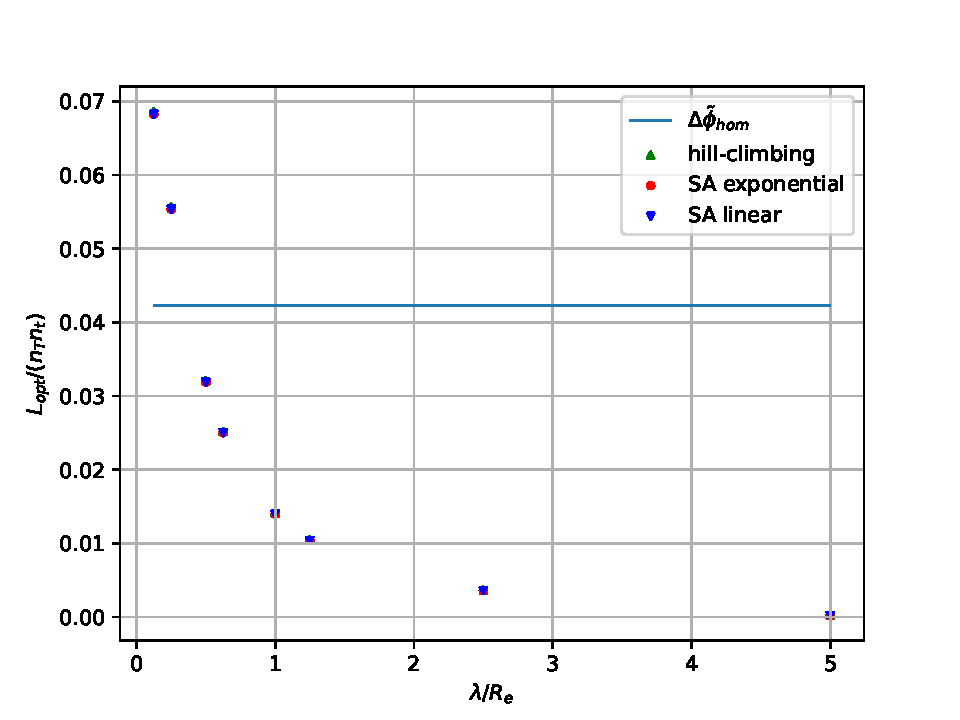
\includegraphics[width=0.6\linewidth]{figures/lamella_opt.pdf}
%     \caption{Minimum of loss function as a function of the lamella periodicity for different optimization schemes, each points is averaged over 100 randomly generated initial configurations.  The initial SA temperature is set to $T_0=1.0\,.$ The exponential cooling scheme is $T_k=T_0 0.85^k$ until $T=T_f=0.001$ and the linear cooling scheme is $T_k=T_0-0.1k$ until $T=T_f=0.0\,.$ $\Delta\tilde\phi_{hom}$ denotes the variance of the composition at the boundaries for the homogeneous system.}
%     \label{fig:lamella_opt}
% \end{figure}

% The values corresponding to different optimization schemes are virtually indistinguishable, the SA schemes do not find a better minimum than the hill-climbing algorithm.


% \subsection{Checkerboard-like target composition}

% \begin{figure}[h]
%     \centering
%     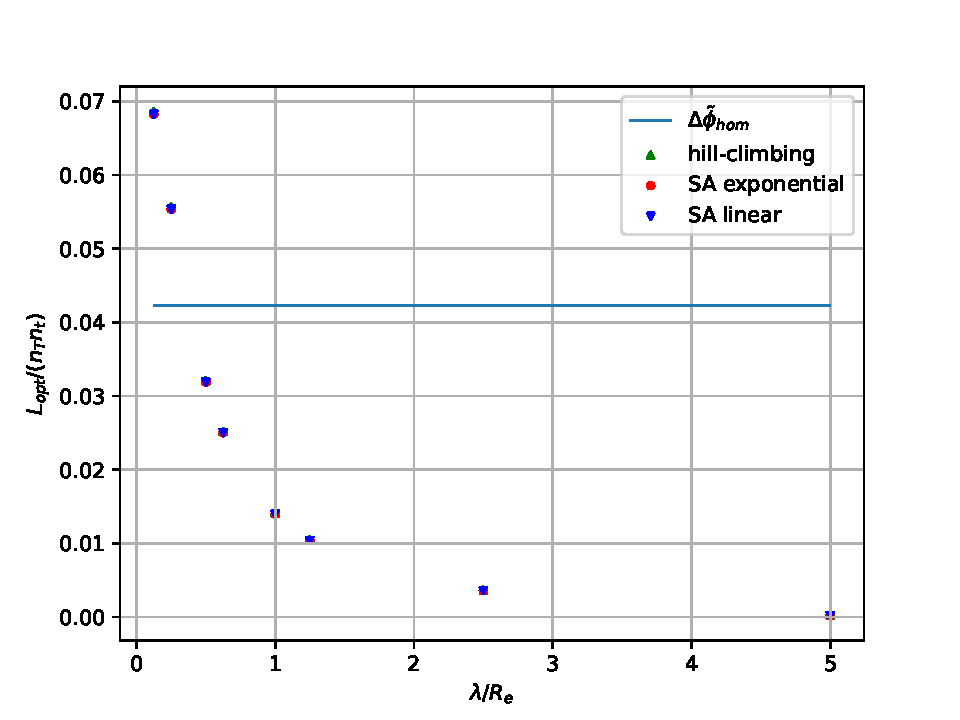
\includegraphics[width=0.6\linewidth]{figures/lamella_opt.pdf}
%     \caption{Minimum of loss function as a function of the checkerboard periodicity for different optimization schemes, each points is averaged over 100 randomly generated initial configurations.  The initial SA temperature is set to $T_0=1.0\,.$ The exponential cooling scheme is $T_k=T_0 0.85^k$ until $T=T_f=0.001$ and the linear cooling scheme is $T_k=T_0-0.1k$ until $T=T_f=0.0\,.$ $\Delta\tilde\phi_{hom}$ denotes the variance of the composition at the boundaries for the homogeneous system.}
%     \label{fig:checkerboard_opt}
% \end{figure}

\newpage
\section{Structure factor}

\begin{itemize}
    \item From here on, only use SD algorithm
    \item Target density over whole system, compare collective structure factor before and after optimization
\end{itemize}

The collective structure factor is \cite{Reister02}:

\begin{align}
    S_\text{coll}(\mathbf q)=\rho_0\int_Vd^3\mathbf r\exp(i\mathbf{qr})P_\text{coll}(\mathbf r)\,,
\end{align}
 
where $P_\text{coll}(\mathbf r)$ is the auto-correlation of the density:

\begin{align}
    P_\text{coll}(\mathbf r)=\langle\phi(\mathbf x)\phi(\mathbf x +\mathbf r)\rangle_{\mathbf{x}}\,,
\end{align}
 
where $\mathbf{r}$ is the separation vector, $\mathbf x$ is the position and $\langle .\rangle_\mathbf x$ denotes the ensemble average.
 
\chapter{Outlook}

\begin{itemize}
    \item Still the old version from Einfuehrung ins Wissenschaftliche Arbeiten
\end{itemize}

The collective diffusion coefficient of a symmetric homopolymer mixture under a boundary-driven diffusion flux has been studied. In the future, more sophisticated and time-dependent boundary conditions will be employed to manipulate the behavior of the bulk, with the ultimate goal of simulating smaller sections of a large continuum simulation using particle-based simulations. The key question is whether or not the time evolution of the boundary densities is sufficient to dictate the time-evolution of the densities in the bulk. An approach based purely on center-of-mass-based polymer conversion zones might be problematic due to the extension of the converted chains beyond the boundaries. Simple conversions without changing the position of the beads may also lead to unlikely configurations of the affected polymer, so it might be necessary to let the chain grow into the simulation box, e.g. using the configurational bias method \cite{ConfBias}.
\appendix

\chapter{Algorithms}


\begin{algorithm}
\caption{Get flippable polymers}\label{alg:get_flip_candidates}
\begin{algorithmic}
\State Let $polyIsflippable[n]$ be a new boolean array initialised with $0$'s
\State $n_f\gets 0$
\For{$poly\gets 0$ to $n-1$}
    \For{$monomer\gets 0$ to $N-1$}
        \State $monoCell\gets poly.beads[monomer].cell$
        \If{Target density available for $monoCell$}
            \State $polyIsflippable[poly]\gets 1$
            \State $n_f\gets n_f+1$
            \State \textbf{break}
        \EndIf
    \EndFor
\EndFor
\State Let $polyFlippableIndices[n_f]$ be a new array
\State $i\gets 0$
\For{$poly\gets 0$ to $n-1$}
\Comment{Store indices of flippable polymers to new array}
    \If{$polyIsflippable[poly]==1$}
        \State $polyFlippableIndices[j]\gets poly$
        \State $j\gets j+1$
    \EndIf
\EndFor
\end{algorithmic}
\end{algorithm}

\begin{algorithm}
\caption{Get cell index matrix}\label{alg:get_cell_indices}
\begin{algorithmic}
\State Let $polyCellIndices[n_f][N]$ be a new array initialised with $-1$'s
\For{$i\gets 0$ to $n_f-1$}
\Comment{Loop over flippable polymers}
    \State $poly \gets polymers[polyFlippableIndices[i]]$
    \State let $monoCells[N]$ be a new array
    \State $j\gets 0$
    \For{$monomer\gets 0$ to $N-1$}
        \If{Target density available for $monoCell$}
            \State $monoCells[j]\gets poly.beads[monomer].cell$
            \State $j\gets j+1$
            \State \textbf{break}
        \EndIf
    \EndFor
    \State quicksort($monoCells\,,0\,,j-1$)
    \State $k\gets 0$
    \For{$monomer\gets 0$ to $j-1$}
    \Comment{Find unique cells}
        \If{$monoCells[monomer]\neq monoCells[monomer+1]$}
            \State $polyCellIndices[i][k]\gets monoCells[monomer]$
            \State $k\gets k+1$
        \EndIf
    \EndFor
    \State $polyCellIndices[i][k]\gets monoCells[j-1]$
\EndFor
\end{algorithmic}
\end{algorithm}



\begin{algorithm}
\caption{Get cell number matrix}\label{alg:get_cell_numbers}
\begin{algorithmic}
\State Let $polyCellNum[n_f][m_t][n_t][N]$ be a new array initialised with $0$'s
\For{$i\gets 0$ to $n_f-1$}
\Comment{Loop over flippable polymers}
    \State $poly \gets polymers[polyFlippableIndices[i]]$
    \State $initialPolytype\gets poly.type$
    \For{$polyType\gets 0$ to $n_t-1$}
        \State $poly.type\gets polyType$
        \Comment Temporarily change polymer type
        \For{$monomer\gets 0$ to $N-1$}
            \State $monoCell\gets poly.beads[monomer].cell$
            \State $monoType\gets poly.beads[monomer].type$
            \For{$j\gets 0$ to $N-1$}
            \Comment{Find corresponding entry}
            \If{$polyCellIndices[i][j]==monoCell$}
                \State $polyCellNum[i][polyType][monoType][j]++$ 
                \State \textbf{break}
            \EndIf
            \EndFor
        \EndFor
    \EndFor
    
    \State $poly.type\gets initialPolytype$
    \Comment Restore polymer type
\EndFor
\end{algorithmic}
\end{algorithm}

\begin{algorithm}[H]
\caption{Simulated annealing}\label{alg:sa}
\begin{algorithmic}
\State $S \gets$ current configuration of polymer types
\State $T \gets T_0$
\While{$T>T_f$}
    \State $n_{flip} \gets 0$
    \While{$n_{flip}<n_{max}$}
        \State Generate new configuration $S^*$ by flipping a random polymer
        \State $n_{flip}\gets n_{flip}+1$
        \State $\Delta L\gets L(S^*)-L(S)$
        \State $r\gets$ random number between 0 and 1
        \If{$r<\exp(-\frac{\Delta L}{T})$}
            \State $S\gets S^*$
        \EndIf
    \EndWhile
\State $T\gets\alpha*T$ \Comment{or different cooling schedule}
\EndWhile
\end{algorithmic}
\end{algorithm}

\chapter{Optimization problem}

\begin{figure}[h]
  \centering
  \begin{subfigure}[b]{0.3\textwidth}
      \centering
      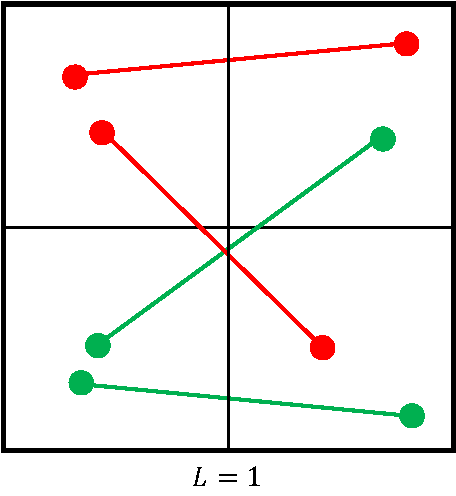
\includegraphics[width=\textwidth]{figures/loss-1.pdf}
      \caption{}
      \label{fig:loss-1}
  \end{subfigure}
    \hfill
  \begin{subfigure}[b]{0.3\textwidth}
      \centering
      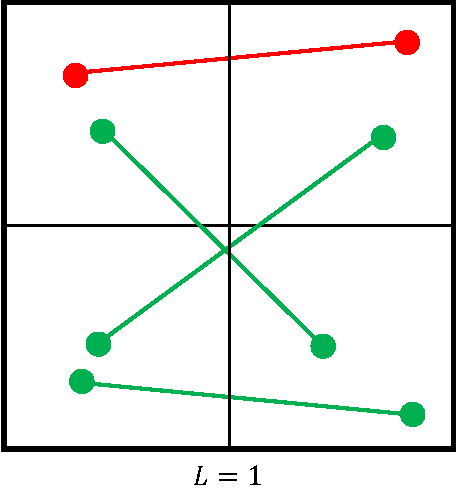
\includegraphics[width=\textwidth]{figures/loss-2.pdf}
      \caption{}
      \label{fig:loss-2}
  \end{subfigure}
      \hfill
  \begin{subfigure}[b]{0.3\textwidth}
      \centering
      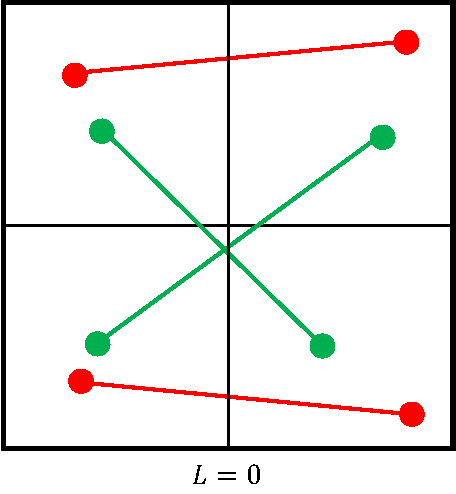
\includegraphics[width=\textwidth]{figures/loss-3.pdf}
      \caption{}
      \label{fig:loss-3}
  \end{subfigure}
     \caption{Example for $n=4$ homopolymers with $N=2$ on a $2\times 2$ grid to show that the loss function defined by $\eqref{eq:lossfunction}$ is in general non-convex in the polymer type configurations, where a neighbouring solution is defined as a configuration of polymer types, where only a single polymer type is changed. Different colours denote different types. The target compositions are $\tilde\phi_{\text A,T}=\tilde\phi_{\text B,T}=0.5$ for all cells. In (a), any possible flip will not lead to a better value of $L\,.$ (b) shows the configuration after conversion of a red polymer to a green one. A flip of the lower polymer now leads to a decrease of the loss function, as shown in (c). Note that this minimum is not unique, since a flip of every polymer would also yield $L=0\,.$}
     \label{fig:loss}
\end{figure}





% \cleardoublepage
%% Bibliographie. Das Argument muss der Name der BIBTeX-Datenbank stehen.
%% Ein Beispiel fuer eine solche Datenbank finden Sie in bthesis_datenbank.bib
\bibliography{bthesis_datenbank} 

% \chapter*{Danksagung}
% Dank\dots

% %% Dieser Befehl MUSS am Ende stehen und erzeugt die Erklaerung ueber die
% %% benutzten Mittel
% \Declaration
\end{document}
